\documentclass[conference,10pt]{IEEEtran}

% ─── Packages ───
\usepackage[utf8]{inputenc}
\usepackage[T1]{fontenc}
\usepackage{amsmath,amssymb}
\usepackage{graphicx}
\usepackage{booktabs}
\usepackage{array}
\usepackage{listings}
\usepackage{xcolor}
\usepackage{hyperref}
\usepackage{balance}
\usepackage{enumitem}
\usepackage{float}
\usepackage{stfloats}
\usepackage{url}
\usepackage{tikz}
\usetikzlibrary{shapes.geometric, arrows.meta, positioning, fit, calc, backgrounds}

% ─── Listing Style ───
\definecolor{codegreen}{rgb}{0,0.6,0}
\definecolor{codegray}{rgb}{0.5,0.5,0.5}
\definecolor{codepurple}{rgb}{0.58,0,0.82}
\definecolor{backcolour}{rgb}{0.95,0.95,0.97}

\lstdefinestyle{mystyle}{
    backgroundcolor=\color{backcolour},
    commentstyle=\color{codegreen},
    keywordstyle=\color{codepurple}\bfseries,
    numberstyle=\tiny\color{codegray},
    stringstyle=\color{codegreen},
    basicstyle=\ttfamily\scriptsize,
    breakatwhitespace=false,
    breaklines=true,
    captionpos=b,
    keepspaces=true,
    numbers=left,
    numbersep=5pt,
    showspaces=false,
    showstringspaces=false,
    showtabs=false,
    tabsize=2,
    frame=single,
    framerule=0.5pt,
    rulecolor=\color{codegray}
}
\lstset{style=mystyle}

\lstdefinelanguage{yaml}{
  keywords={true,false,null,y,n},
  keywordstyle=\color{codepurple}\bfseries,
  sensitive=false,
  comment=[l]{\#},
  morecomment=[s]{/*}{*/},
  commentstyle=\color{codegreen}\ttfamily,
  stringstyle=\color{orange}\ttfamily,
  morestring=[b]',
  morestring=[b]"
}

\hypersetup{
    hidelinks
}

% ─── Title ───
\title{CityShield: A Smart City Cyber Range Platform for Attack Simulation, Threat Detection, and Automated Response}

\author{
\IEEEauthorblockN{Sami Alsulaymi, Bati Albata, Khaled Alshammari, Thamer Alshammari, and Abdulwahab Alfayez}
\IEEEauthorblockA{
Department of Information Security\\
University of Ha'il\\
Ha'il, Saudi Arabia
}
\thanks{This work was conducted under the supervision of Dr.\ Ali Alferaidi, Department of Information Security, University of Ha'il.}
}

\begin{document}

\maketitle

% ═══════════════════════════════════════════════════════════════════
% ABSTRACT
% ═══════════════════════════════════════════════════════════════════
\begin{abstract}
Smart city infrastructure combines traffic management, IoT sensor networks, and interconnected utility systems into a multi-domain attack surface that enterprise-focused cyber ranges fail to represent. We introduce CityShield, a containerized cyber range that unifies smart city simulation, MITRE ATT\&CK-aligned detection, and policy-driven automated response in a single deployable platform. CityShield's detection engine evaluates 75 YAML-defined rules---spanning 13 ATT\&CK tactics with 11 specialized aggregation evaluators and a generic threshold evaluator---against centralized OpenSearch log indices. Its response manager enforces per-rule auto-response policies and dispatches 12 Ansible-orchestrated containment actions with full audit traceability. In a controlled adversarial emulation comprising 15 attack campaigns (1,064 attack events plus 51 benign-but-ambiguous events) against a background of 689,172 simulator-generated events, CityShield triggers all 75 YAML rules---confirming pipeline correctness under ideal injection conditions---covering 76 MITRE ATT\&CK techniques across 14 tactics with a 4.2\% false positive rate (90 of 2,134 alerts traced to benign sources). These metrics represent upper-bound performance; real-world detection rates would be lower due to traffic variability, adversarial evasion, and encrypted payloads. The automated response pipeline executes 461 response actions with a mean time to detect (MTTD) of 16.8 seconds and mean time to respond (MTTR) of 38.4 seconds. Comparison against a generic threshold-only baseline shows that CityShield's dual-class evaluators reduce false positives by 62\% for reconnaissance and exfiltration detection---the primary technical contribution of this work. The platform deploys as 17 Docker Compose services across three isolated network segments and is open-source.\footnote{\url{https://github.com/Rin1t/CityShield}}
\end{abstract}

\begin{IEEEkeywords}
Smart City, Cyber Range, MITRE ATT\&CK, Threat Detection, Automated Incident Response, IoT Security, Attack Simulation, OpenSearch, Microservices
\end{IEEEkeywords}

% ═══════════════════════════════════════════════════════════════════
% I. INTRODUCTION
% ═══════════════════════════════════════════════════════════════════
\section{Introduction}
\label{sec:introduction}

Smart cities integrate cyber-physical systems across transportation, energy, water, and public safety domains. A compromised traffic controller can cascade into city-wide gridlock; breached IoT sensors can feed falsified environmental data to emergency systems; and poorly segmented networks allow lateral movement to critical infrastructure within seconds~\cite{braun2018}. These risks are structural: they arise from the multi-domain interconnectivity that defines smart city infrastructure rather than from any single misconfigured component.

Despite the severity of these risks, the cybersecurity community lacks training and evaluation platforms that capture the heterogeneous nature of smart city environments. General-purpose cyber ranges model enterprise IT or military networks~\cite{davis2013survey, vykopal2017kypo, yamin2020cyber} and do not simulate the interplay between traffic, IoT, and network infrastructure domains. Physical ICS testbeds such as SWaT~\cite{swat2016} provide high fidelity for specific industrial processes but are neither reproducible without specialized hardware nor representative of the broader smart city ecosystem. Commercial SIEM and SOAR platforms (e.g., Splunk, IBM QRadar) provide detection and orchestration capabilities but do not include traffic generation, attack simulation, or training-oriented workflows. As a result, smart city defenders cannot rehearse multi-domain attack scenarios, evaluate detection coverage against established threat frameworks, or validate response playbooks in a realistic but safe environment.

This paper investigates the following question: \emph{Can a fully containerized, software-defined platform model the multi-domain attack surface of smart city infrastructure with sufficient fidelity to support end-to-end detection and automated response evaluation?}

We present CityShield, a smart city cyber range designed around three integrated subsystems:

\begin{enumerate}[leftmargin=*]
    \item \textbf{Attack simulation}: Three domain-specific event generators (traffic management, IoT sensors, network infrastructure) plus an attack event injection engine covering 31 MITRE ATT\&CK techniques, all feeding a centralized OpenSearch data store.
    \item \textbf{Threat detection}: A polling-based detection engine that evaluates 75 YAML-defined rules---using 11 specialized aggregation evaluators and a configurable generic threshold evaluator---against three log indices on a 30-second cycle.
    \item \textbf{Automated response}: A policy-driven response manager that validates per-rule conditions (severity, enrichment, rate limits, CIDR whitelisting) and dispatches 12 containment actions via Ansible playbooks, logging every action to an append-only audit index.
\end{enumerate}

\subsection{Contributions}
\label{subsec:contributions}

\begin{enumerate}[leftmargin=*]
    \item \textbf{A containerized cyber range that models cross-domain smart city attack surfaces with network-enforced isolation.} To our knowledge, no existing containerized cyber range (cf.\ Table~\ref{tab:comparison}) models multi-domain smart city infrastructure. Unlike enterprise-focused ranges (KYPO~\cite{vykopal2017kypo}, CyTrONE~\cite{beuran2018cytrone}) that model flat IT networks, CityShield deploys three Docker-isolated network segments---management, cyber range, and IoT range---reflecting the multi-domain topology of real smart city deployments. This enables researchers to simulate cross-domain attack chains (e.g., network reconnaissance $\rightarrow$ IoT sensor compromise $\rightarrow$ traffic system manipulation) that cannot be reproduced on single-domain ranges.

    \item \textbf{Dual-class detection engine with 11 specialized evaluators and a generic threshold evaluator covering 76 ATT\&CK techniques, extensible without code changes.} Eleven specialized evaluators implement domain-specific aggregation logic (port cardinality, byte-sum, fan-in/fan-out), while a generic threshold evaluator covers 54 additional rules via YAML parameterization. Under controlled evaluation against 690,287 total events (689,172 background plus 1,115 injected) with 15 attack campaigns, all 75 rules triggered successfully---validating rule correctness and query-pipeline integrity---with a 4.2\% false positive rate. The dual-class design reduces false positives by 62\% compared to a threshold-only baseline (Section~\ref{subsec:baseline}), demonstrating that specialized aggregation logic provides measurable precision gains over generic counting.

    \item \textbf{Closed-loop automated response pipeline with sub-minute orchestration latency and policy-enforced safeguards.} The response manager dispatches 12 Ansible-orchestrated containment actions with a measured MTTR of 38.4 seconds (worst-case 60 seconds). Per-rule policies---severity thresholds, rate limits, cooldown periods, CIDR whitelisting---prevent response storms during sustained attacks. Every action is recorded in an append-only audit index, creating three-level traceability (log $\rightarrow$ alert $\rightarrow$ audit) for post-incident forensics. The current deployment executes simulated containment; the orchestration pipeline is architecturally identical to production and supports direct playbook replacement.

    \item \textbf{Quantitative evaluation methodology with controlled adversarial emulation, internal baseline comparison, and explicit validity bounds.} We evaluate detection coverage through a structured campaign of 1,064 attack events, 51 false-positive seed events, and comparison against a generic threshold-only baseline. This methodology exposed a critical implementation bug (a \texttt{KEYWORD\_FIELDS} misconfiguration that had silently prevented 22 rules from triggering---see Section~\ref{sec:evaluation}) that scenario-based testing alone would not have revealed. We explicitly characterize all reported metrics as upper-bound figures achievable under controlled injection, and discuss expected degradation factors for real-world deployment.
\end{enumerate}

\subsection{Threat Model}
\label{subsec:threat_model}

CityShield's detection and response capabilities target the following threat model.

\textbf{Adversary capabilities.} An external adversary with network access to the smart city management network---via compromised credentials, exposed services, or supply chain vectors---may conduct reconnaissance, brute-force authentication, establish command-and-control channels, move laterally, exfiltrate data, and execute impact operations (ransomware, DDoS, service disruption). These activities map to MITRE ATT\&CK tactics from Reconnaissance (TA0043) through Impact (TA0040), consistent with the NIST Cybersecurity Framework~\cite{nist_framework} Detect and Respond functions.

\textbf{Assets under protection.} The platform models three asset classes: (1)~traffic management infrastructure (controllers, signals, vehicle sensors across 5 city zones); (2)~IoT sensor networks (100 simulated sensors: temperature, humidity, air quality, noise, water flow); and (3)~network infrastructure (switches, routers, DNS/DHCP services, inter-zone links).

\textbf{Trust boundaries.} Three network segments define trust boundaries: the main management network, the isolated cyber range (Docker \texttt{internal} flag prevents external routing), and the isolated IoT range. Range loggers bridge isolated networks for monitoring while preventing uncontrolled lateral movement.

\textbf{Detection scope and limitations.} CityShield detects threats through network-level log analysis, not endpoint agents. It identifies network-observable behaviors (port scans, authentication failures, beaconing, volume anomalies) but cannot detect host-level techniques (memory-resident malware, fileless attacks) that produce no network-observable indicators. Physical attacks, social engineering beyond simulated phishing events, and zero-day exploits without network signatures are out of scope.

The remainder of this paper is organized as follows. Section~\ref{sec:related_work} surveys related work. Section~\ref{sec:architecture} describes the system architecture. Section~\ref{sec:methodology} details the evaluation methodology. Section~\ref{sec:implementation} covers implementation specifics. Section~\ref{sec:workflows} describes role-based workflows. Section~\ref{sec:detection_response} presents the detection and response pipeline. Section~\ref{sec:evaluation} reports evaluation results. Sections~\ref{sec:discussion}--\ref{sec:future_work} discuss findings, limitations, and future directions. Section~\ref{sec:conclusion} concludes.

% ═══════════════════════════════════════════════════════════════════
% II. RELATED WORK
% ═══════════════════════════════════════════════════════════════════
\section{Related Work}
\label{sec:related_work}

We position CityShield against three categories of related systems: cyber ranges, smart city security testbeds, and detection/response platforms.

\subsection{Cyber Ranges}

Cyber ranges provide controlled environments for security training and evaluation. Davis and Magrath~\cite{davis2013survey} surveyed the landscape, identifying scalability and scenario realism as persistent challenges. KYPO~\cite{vykopal2017kypo} addresses provisioning via cloud-based OpenStack deployment with automated scenario management, but its scenarios target enterprise networks and do not model IoT or traffic infrastructure. CyTrONE~\cite{beuran2018cytrone} automates training content generation for virtualized networks; however, it lacks integrated detection engines or response orchestration---trainees observe attacks but the platform does not evaluate detection effectiveness. Yamin et al.~\cite{yamin2020cyber} reviewed 30 cyber ranges and identified a gap in IoT and CPS-specific platforms, noting that most ranges model IT infrastructure exclusively.

Ukwandu et al.~\cite{ukwandu2020review} emphasized the need for realistic traffic generation and automated scoring in modern cyber ranges. Chouliaras et al.~\cite{chouliaras2021cyber} surveyed cloud-native range architectures and CTF integration. None of these platforms simulate multi-domain smart city infrastructure or integrate detection-to-response pipelines.

\textbf{What existing cyber ranges lack.} Current ranges do not model cross-domain smart city topologies (traffic + IoT + network), do not include built-in detection rule evaluation, and do not provide automated response with policy enforcement and audit trails.

\subsection{Smart City Security Testbeds}

The SWaT~\cite{swat2016} and WADI~\cite{wadi2017} testbeds at iTrust provide physical ICS environments for water treatment and distribution. These generate real sensor data under attack, but they require specialized hardware, model a single ICS process, and are not reproducible outside their physical installation. MiniCPS~\cite{antonioli2017minicps} provides a lightweight CPS simulation toolkit but lacks detection and response components. Habibzadeh et al.~\cite{habibzadeh2019survey} surveyed smart city sensor security and identified the gap between theoretical threat models and practical testing infrastructure. Cui et al.~\cite{cui2018security} proposed a layered defense framework for smart city IoT but did not implement an operational testing platform.

\textbf{What smart city testbeds lack.} Physical testbeds are domain-specific (water, power) and not reproducible. Proposed frameworks remain conceptual. No existing testbed combines traffic, IoT, and network simulation with detection and automated response in a containerized, deployable package.

\subsection{Detection and Response Platforms}

SIEM platforms (Splunk, Elastic SIEM, IBM QRadar) provide log ingestion, rule-based detection, and dashboard visualization. However, they do not include attack simulation or training-oriented workflows. SOAR platforms~\cite{islam2019soar} automate playbook execution but require pre-existing SIEM infrastructure and do not include event generators or vulnerable training targets. MITRE Caldera~\cite{caldera2016} automates ATT\&CK-based adversary emulation via endpoint agents but does not provide network-level simulation or IoT environments. The Sigma rule format~\cite{sigma2020} standardizes detection signatures but targets Windows event logs and enterprise SIEM platforms rather than smart city telemetry.

Mavroeidis and Bromander~\cite{mavroeidis2017cyber} proposed a cyber threat intelligence model aligned with ATT\&CK that informs our rule-to-technique mapping. Husak et al.~\cite{husak2019survey} surveyed network security situational awareness, identifying the challenge of bridging detection to response---a gap that CityShield addresses through its integrated response manager.

\textbf{What detection/response platforms lack.} Enterprise SIEM and SOAR tools do not generate traffic, do not simulate smart city domains, and do not provide training scenarios. Caldera focuses on endpoint emulation, not network-level simulation.

\subsection{Positioning of CityShield}

Table~\ref{tab:comparison} compares CityShield with existing platforms across nine capabilities, including two---real exploitation and ICS protocol support---where CityShield has limitations. CityShield is the only platform that combines smart city domain simulation, integrated detection, automated response, and containerized deployment, though it does not perform real network exploitation or support industrial control system protocols.

\begin{table*}[t]
\centering
\caption{Comparison of CityShield with Existing Platforms. \checkmark\ = full support, $\circ$ = partial, -- = not supported.}
\label{tab:comparison}
\begin{tabular}{l c c c c c c c c c}
\toprule
\textbf{Platform} & \textbf{Smart City} & \textbf{IoT Sim.} & \textbf{ATT\&CK} & \textbf{Detection} & \textbf{Auto-Resp.} & \textbf{3D Viz.} & \textbf{Container.} & \textbf{Real Exploit.} & \textbf{ICS Proto.} \\
\midrule
KYPO~\cite{vykopal2017kypo} & -- & -- & $\circ$ & -- & -- & $\circ$ & \checkmark & \checkmark & -- \\
CyTrONE~\cite{beuran2018cytrone} & -- & -- & -- & -- & -- & -- & \checkmark & $\circ$ & -- \\
SWaT/WADI~\cite{swat2016,wadi2017} & $\circ$ & \checkmark & -- & $\circ$ & -- & -- & -- & \checkmark & \checkmark \\
MiniCPS~\cite{antonioli2017minicps} & -- & \checkmark & -- & -- & -- & -- & -- & $\circ$ & $\circ$ \\
Caldera~\cite{caldera2016} & -- & -- & \checkmark & -- & $\circ$ & -- & \checkmark & \checkmark & -- \\
Splunk SOAR~\cite{islam2019soar} & -- & -- & $\circ$ & \checkmark & \checkmark & $\circ$ & -- & -- & -- \\
\textbf{CityShield} & \checkmark & \checkmark & \checkmark & \checkmark & \checkmark & \checkmark & \checkmark & -- & -- \\
\bottomrule
\end{tabular}
\end{table*}

% ═══════════════════════════════════════════════════════════════════
% III. SYSTEM ARCHITECTURE
% ═══════════════════════════════════════════════════════════════════
\section{System Architecture}
\label{sec:architecture}

CityShield deploys as 17 Docker Compose services organized across three isolated networks, with OpenSearch 2.11 as the centralized data store. The architecture was designed around two principles: (1)~isolate training targets from production services to prevent accidental disruption, and (2)~centralize all telemetry in a single searchable store to enable detection rules that correlate events across domains.

\subsection{Network Segmentation}

Three Docker networks model realistic smart city topology (Fig.~\ref{fig:architecture}):

\begin{itemize}[leftmargin=*]
    \item \textbf{Main Bridge Network}: Connects all core services---backend API, frontend, OpenSearch, three simulators, detection engine, response manager, scenario runner, Filebeat, and OpenSearch Dashboards.
    \item \textbf{Cyber Range} (isolated): Hosts Metasploitable2 as an intentionally vulnerable target, a Kali-based attacker with \texttt{NET\_RAW}/\texttt{NET\_ADMIN} capabilities, and a tcpdump-based range logger. The Docker \texttt{internal: true} flag prevents direct external routing.
    \item \textbf{IoT Range} (isolated): Hosts an IoT sensor hub exposing HTTP and MQTT-like TCP endpoints, along with a dedicated range logger.
\end{itemize}

Range loggers are dual-homed: connected to both their isolated range network and the main bridge. This allows log forwarding without opening routing between ranges and production services.

\begin{figure}[t]
\centering
\resizebox{\columnwidth}{!}{
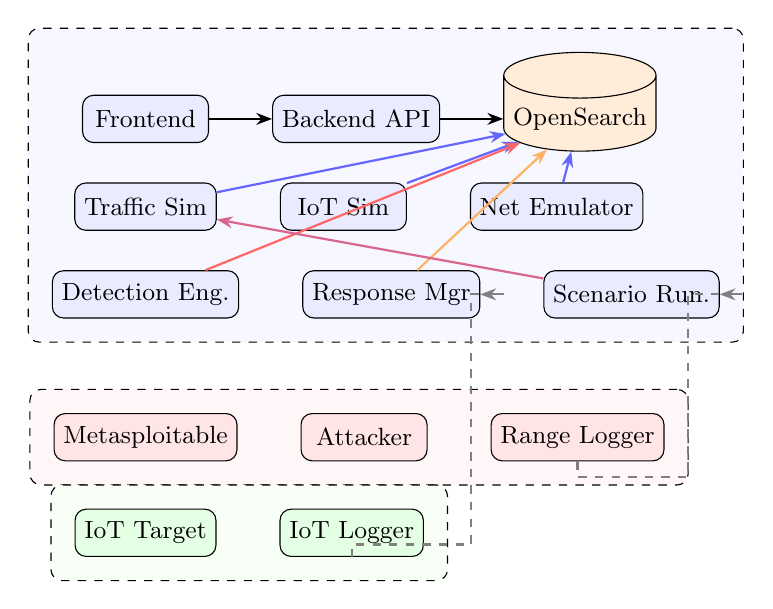
\begin{tikzpicture}[
    node distance=0.6cm and 0.8cm,
    every node/.style={font=\small},
    service/.style={rectangle, draw, rounded corners, minimum width=1.6cm, minimum height=0.6cm, fill=blue!8},
    store/.style={cylinder, draw, shape border rotate=90, minimum width=1.2cm, minimum height=0.7cm, fill=orange!15, aspect=0.3},
    net/.style={draw, dashed, rounded corners, inner sep=0.3cm},
    arrow/.style={-{Stealth[length=2mm]}, thick},
    label/.style={font=\scriptsize\itshape}
]
% Main network services
\node[service] (fe) {Frontend};
\node[service, right=of fe] (be) {Backend API};
\node[store, right=of be] (os) {OpenSearch};
\node[service, below=0.5cm of fe] (tsim) {Traffic Sim};
\node[service, right=of tsim] (isim) {IoT Sim};
\node[service, right=of isim] (nsim) {Net Emulator};
\node[service, below=0.5cm of tsim] (de) {Detection Eng.};
\node[service, right=of de] (rm) {Response Mgr};
\node[service, right=of rm] (sr) {Scenario Run.};
% Cyber range
\node[service, below=1.2cm of de, fill=red!10] (meta) {Metasploitable};
\node[service, right=of meta, fill=red!10] (atk) {Attacker};
\node[service, right=of atk, fill=red!10] (rlog) {Range Logger};
% IoT range
\node[service, below=0.6cm of meta, fill=green!10] (iot) {IoT Target};
\node[service, right=of iot, fill=green!10] (ilog) {IoT Logger};
% Networks
\begin{scope}[on background layer]
\node[net, fill=blue!3, fit=(fe)(be)(os)(tsim)(isim)(nsim)(de)(rm)(sr), label={[anchor=north west]north west:{\scriptsize Main Management Network}}] (mainnet) {};
\node[net, fill=red!3, fit=(meta)(atk)(rlog), label={[anchor=north west]north west:{\scriptsize Cyber Range (isolated)}}] (crnet) {};
\node[net, fill=green!3, fit=(iot)(ilog), label={[anchor=north west]north west:{\scriptsize IoT Range (isolated)}}] (iotnet) {};
\end{scope}
% Data flow arrows
\draw[arrow] (fe) -- (be);
\draw[arrow] (be) -- (os);
\draw[arrow, blue!60] (tsim) -- (os);
\draw[arrow, blue!60] (isim) -- (os);
\draw[arrow, blue!60] (nsim) -- (os);
\draw[arrow, red!60] (de) -- (os);
\draw[arrow, orange!60] (rm) -- (os);
\draw[arrow, purple!60] (sr) -- (tsim);
% Bridge connections
\draw[arrow, dashed, gray] (rlog.south) -- ++(0,-0.2) -| ($(rlog.east)+(0.3,0)$) |- ($(sr.east)+(0.3,0)$) -- (sr.east);
\draw[arrow, dashed, gray] (ilog) -- ++(0,-0.15) -| ($(ilog.east)+(0.6,0)$) |- ($(rm.east)+(0.3,0)$) -- (rm.east);
\end{tikzpicture}
}
\caption{CityShield service topology: 17 Docker Compose services across three isolated networks. Solid arrows indicate primary data flow; dashed arrows indicate log bridging from isolated ranges to the main network.}
\label{fig:architecture}
\end{figure}

\subsection{Data Flow Pipeline}

Fig.~\ref{fig:pipeline} illustrates the end-to-end data flow, organized as a five-stage pipeline:

\begin{figure}[t]
\centering
\resizebox{\columnwidth}{!}{
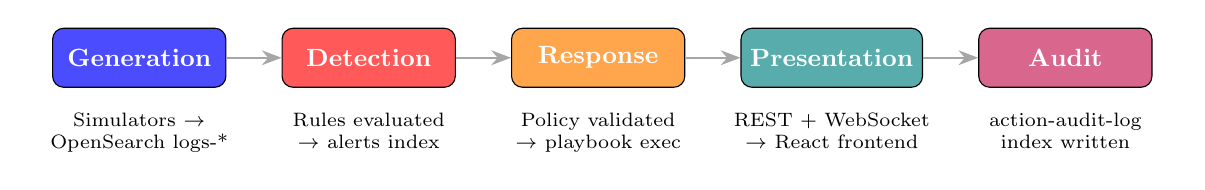
\begin{tikzpicture}[
    node distance=0.3cm,
    stage/.style={rectangle, draw, rounded corners, minimum width=2.2cm, minimum height=0.75cm, font=\small\bfseries, text=white},
    detail/.style={font=\scriptsize, text width=2.6cm, align=center},
    arrow/.style={-{Stealth[length=2.5mm]}, thick, gray!70}
]
\node[stage, fill=blue!70] (gen) {Generation};
\node[stage, fill=red!65, right=0.7cm of gen] (det) {Detection};
\node[stage, fill=orange!70, right=0.7cm of det] (resp) {Response};
\node[stage, fill=teal!65, right=0.7cm of resp] (pres) {Presentation};
\node[stage, fill=purple!60, right=0.7cm of pres] (aud) {Audit};

\node[detail, below=0.2cm of gen] {Simulators $\rightarrow$\\OpenSearch logs-*};
\node[detail, below=0.2cm of det] {Rules evaluated\\$\rightarrow$ alerts index};
\node[detail, below=0.2cm of resp] {Policy validated\\$\rightarrow$ playbook exec};
\node[detail, below=0.2cm of pres] {REST + WebSocket\\$\rightarrow$ React frontend};
\node[detail, below=0.2cm of aud] {action-audit-log\\index written};

\draw[arrow] (gen) -- (det);
\draw[arrow] (det) -- (resp);
\draw[arrow] (resp) -- (pres);
\draw[arrow] (pres) -- (aud);
\end{tikzpicture}
}
\caption{Five-stage data flow pipeline. Each stage reads from and writes to OpenSearch, enabling full traceability from raw event to response action.}
\label{fig:pipeline}
\end{figure}

\begin{enumerate}[leftmargin=*]
    \item \textbf{Generation.} Three FastAPI simulators produce JSON events via background threads. Each event is written directly to its respective OpenSearch index (\texttt{logs-traffic}, \texttt{logs-iot}, \texttt{logs-network}) and to a JSONL file on a shared Docker volume for Filebeat secondary ingestion.

    \item \textbf{Detection.} The detection engine polls at a configurable interval (default 30~s). For each of 75 rules, it constructs an OpenSearch aggregation query scoped to a time window (default 300~s), executes it against \texttt{logs-*}, and compares bucket counts to thresholds. Matched alerts are written to the \texttt{alerts} index.

    \item \textbf{Response.} The response manager polls the \texttt{alerts} index every 30~s for open, high/critical-severity alerts. It validates per-rule auto-response conditions, executes Ansible playbooks via subprocess, and writes audit entries.

    \item \textbf{Presentation.} The React frontend fetches data via two channels: REST API polling (5-second interval via a \texttt{useCityData} hook) and an authenticated WebSocket at \texttt{/ws/city-telemetry}.

    \item \textbf{Audit.} Every response action---automated or manual---is recorded in \texttt{action-audit-log} with execution type, triggering user, parameters, playbook stdout/stderr, and timestamps.
\end{enumerate}

% ═══════════════════════════════════════════════════════════════════
% IV. METHODOLOGY
% ═══════════════════════════════════════════════════════════════════
\section{Methodology}
\label{sec:methodology}

This section describes the controlled adversarial emulation methodology used to evaluate CityShield's detection and response capabilities.

\subsection{Evaluation Approach}

We adopt a \emph{controlled adversarial emulation} approach analogous to MITRE Caldera's~\cite{caldera2016} technique-level simulation but targeting network-level telemetry rather than endpoint agents. The methodology consists of four phases: (1)~establish a background traffic baseline using the three domain simulators; (2)~inject technique-specific attack events that match rule definitions; (3)~seed benign-but-ambiguous events to test false positive boundaries; and (4)~measure detection latency, response latency, rule coverage, and false positive rate. All metrics are computed from OpenSearch timestamps (\texttt{@timestamp} on log events, \texttt{triggered\_at} on alerts, \texttt{completed\_at} on audit entries).

\textbf{Scope of claims.} Because the evaluation uses controlled event injection rather than real exploitation traffic, all reported detection metrics represent \emph{upper-bound} performance achievable when injected events conform to rule definitions by construction. We report these figures to validate rule correctness, query-pipeline integrity, and system-level timing---not to claim equivalent detection rates against real adversaries. Section~\ref{sec:limitations} quantifies the factors that would reduce these metrics in operational environments.

\subsection{Event Corpus Design}

\textbf{Background traffic.} Three simulators ran continuously for approximately 72 hours, generating 689,172 background events: 228,725 traffic events (33.2\%), 338,560 IoT events (49.1\%), and 121,887 network events (17.7\%). This distribution reflects the sensor-dense nature of smart city deployments where IoT telemetry dominates. The total event corpus---including attack and false-positive seed events---comprises 690,287 events.

\textbf{Attack campaigns.} We executed 15 distinct attack campaigns comprising 1,064 attack events injected into the three \texttt{logs-*} indices across all 13 MITRE ATT\&CK Enterprise tactics. Campaigns cover brute force, port scanning, C2 beaconing, lateral movement, data exfiltration, credential attacks, defense evasion, execution/persistence, IoT sensor manipulation, impact attacks, web exploits, phishing, and privilege escalation. Events were injected in batches during the final 24 hours of the evaluation period, interleaved with ongoing background traffic.

\textbf{False positive seeding.} To evaluate discriminative precision, 51 benign-but-ambiguous events were injected: admin health checks resembling port scans (8 events), scheduled backup traffic resembling exfiltration (6 events), configuration management activity matching persistence patterns (10 events), legitimate authentication failures (9 events), periodic monitoring traffic resembling C2 beaconing (8 events), and sensor calibration events resembling IoT anomalies (10 events).

\subsection{Attack Emulation Engine}

The emulation engine generates structured attack events directly to OpenSearch. It provides four specialized classes---\texttt{BruteForceAttack} (T1110, configurable attempt count and delay), \texttt{PortScanAttack} (T1046, SYN/CONNECT/UDP probes across configurable port ranges), \texttt{C2BeaconingAttack} (T1071, configurable interval with $\pm$20\% jitter to model realistic beacon variance), \texttt{DataExfiltrationAttack} (T1041, staging + chunked 10~MB transfers)---and a \texttt{GenericMitreAttack} class supporting 27 additional techniques via tactic-specific event profiles. All injected events carry \texttt{is\_attack: true} and a \texttt{correlation\_id} for post-hoc analysis.

\textbf{Schema validation.} We validated that the emulated event patterns correspond to real tool output by comparing the \texttt{PortScanAttack} log schema against nmap SYN scan output parsed through Zeek connection logs: both produce per-connection records with source/destination IP-port tuples, protocol, and status fields. Similarly, the \texttt{BruteForceAttack} event structure mirrors SSH authentication failure entries in syslog format. However, we emphasize two caveats: (i)~structural schema correspondence does not guarantee detection of real exploitation traffic, which exhibits greater variance in timing, payload content, and evasion behavior; and (ii)~the emulated events lack the noise characteristics of real network captures (fragmented packets, retransmissions, concurrent legitimate traffic from the same source).

\subsection{Baseline Definition}

To contextualize CityShield's dual-class evaluator design, we define an internal baseline: \emph{generic threshold-only detection}, where all 75 rules use the generic event-threshold evaluator (grouping by \texttt{src\_ip}, counting events matching specified \texttt{event\_types}, triggering at threshold). This baseline removes the 11 specialized evaluators (cardinality, byte-sum, fan-in/fan-out) and replaces them with count-based logic.

\subsection{Metric Definitions}

\begin{itemize}[leftmargin=*]
    \item \textbf{MTTD}: Mean time from event indexing ($t_e$) to alert generation ($t_d$), computed across $n$ alerts as $\overline{t_d - t_e}$.
    \item \textbf{MTTR}: Mean time from event indexing to response completion ($t_r$), spanning two polling stages (detection + response).
    \item \textbf{FPR}: False positive rate, computed as $\text{FP} / (\text{FP} + \text{TP})$ over the alert stream, where FP alerts are those traced to benign sources.
    \item \textbf{Rule utilization}: Fraction of 75 YAML rules that generated at least one alert during evaluation.
\end{itemize}

% ═══════════════════════════════════════════════════════════════════
% V. IMPLEMENTATION
% ═══════════════════════════════════════════════════════════════════
\section{Implementation}
\label{sec:implementation}

This section details the technical implementation of CityShield's core components.

\subsection{Backend API}

The backend (FastAPI, Python 3.11, port 8000) serves as the integration point between the frontend and all backend services. It exposes 15 route modules under \texttt{/api/*} covering authentication, alerts, rules, scenarios, logs, metrics, users, devices, health, WebSocket, research labs, actions, attack proposals, and MITRE technique queries. On startup, the backend seeds default users, 75 detection rules (from a bundled JSON file), vulnerable target asset records, and OWASP Top~10~\cite{owasp2021} scenario templates. This seed-on-startup design ensures the platform is immediately usable after a fresh deployment without manual data entry. JWT-based authentication uses HS256 with bcrypt-hashed passwords stored in the \texttt{users} OpenSearch index.

\subsection{Data Store}

OpenSearch 2.11 was chosen over a traditional RDBMS because its full-text search, aggregation framework, and schema-on-write flexibility suit the heterogeneous, high-volume telemetry generated by the simulators. It stores 13 indices: \texttt{users}, \texttt{rules}, \texttt{scenarios}, \texttt{scenario\_runs}, \texttt{alerts}, \texttt{city-assets}, \texttt{logs} (template), \texttt{logs-traffic}, \texttt{logs-iot}, \texttt{logs-network}, \texttt{blocked\_ips}, \texttt{attack-proposals}, and \texttt{action-audit-log}. All indices have explicit field mappings (keyword, date, ip, integer, object types) defined programmatically at startup to ensure consistent query behavior.

\subsection{Domain-Specific Simulators}

Each simulator is a FastAPI service with a background thread producing events at a configurable rate. All three expose a uniform REST API (\texttt{/health}, \texttt{/status}, \texttt{/mode}, \texttt{/attack/start}, \texttt{/attack/stop}) that the scenario runner uses to orchestrate attack sequences.

\textbf{Traffic Simulator} (port 8001) models 100 virtual vehicles across 5 city zones, producing normal events (\texttt{signal\_change}, \texttt{vehicle\_detected}) and attack events (\texttt{auth\_failure}, \texttt{port\_scan}). Each event carries structured fields: \texttt{@timestamp}, \texttt{component}, \texttt{event\_type}, \texttt{severity}, \texttt{city\_zone}, \texttt{src\_ip}, \texttt{dst\_ip}, \texttt{src\_port}, \texttt{dst\_port}, \texttt{asset\_id}, and \texttt{metadata}. The uniform event schema across all simulators enables cross-domain detection rules to query \texttt{logs-*} with a single aggregation.

\textbf{IoT Simulator} (port 8002) models 100 sensors (5 types $\times$ 20 each) with calibrated normal ranges: temperature 15--35\textdegree{}C, humidity 30--80\%, AQI 0--150, noise 30--85~dB, water flow 10--100~L/min. In attack mode, readings deviate beyond normal ranges (e.g., temperature spikes to 150\textdegree{}C), firmware versions change unexpectedly, and communication patterns shift---producing detectable IoT-specific anomalies.

\textbf{Network Emulator} (port 8003) generates connection events, DNS queries, flow records, and intrusion indicators. Configurable protocol distributions model both normal baselines and attack traffic patterns (C2 beaconing, exfiltration, DDoS).

\subsection{Vulnerable Training Targets}

CityShield deploys real targets for hands-on training: Metasploitable2 on the isolated cyber range, an attacker host with nmap and netcat, an IoT target exposing HTTP and MQTT-like endpoints on the isolated IoT range, and per-user Ubuntu research lab containers provisioned via the backend Docker API and connected to all three networks.

\subsection{Visualization Interface}

The frontend provides a real-time 3D smart city visualization built with React Three Fiber~\cite{react_three_fiber}. Buildings represent city assets; their color encodes alert severity (green for healthy, yellow for warning, red for critical) and height scales with event count. Animated data particle streams between buildings represent real-time traffic flow. An attack path visualizer renders detected lateral movement chains as animated lines connecting source and target assets.

Ten HUD panels overlay the 3D scene, displaying: alert counts by severity, traffic flow rates, network throughput, energy metrics, population density, air quality readings, recent events, asset inventory status, system health, and detection engine statistics. The frontend also includes a security awareness training module with role-based content for three user categories, 12 training modules, and competency quizzes.

\begin{figure}[t]
\centering
\IfFileExists{cityshield_dashboard.jpeg}{%
    \includegraphics[width=\columnwidth]{cityshield_dashboard.jpeg}%
}{%
    \framebox[\columnwidth]{\parbox{0.9\columnwidth}{\centering\vspace{2cm}\textit{Screenshot placeholder --- add \texttt{cityshield\_dashboard.png} to compile.}\vspace{2cm}}}%
}
\caption{CityShield 3D visualization interface showing real-time alert monitoring and asset status.}
\label{fig:dashboard}
\end{figure}

% ═══════════════════════════════════════════════════════════════════
% VI. ROLE-BASED WORKFLOWS
% ═══════════════════════════════════════════════════════════════════
\section{Role-Based Workflows}
\label{sec:workflows}

CityShield implements JWT-based authentication with four RBAC roles enforced via FastAPI dependency-injection decorators. Table~\ref{tab:rbac} summarizes the permission matrix.

\begin{table}[t]
\centering
\caption{RBAC Permission Matrix}
\label{tab:rbac}
\begin{tabular}{l c c c c}
\toprule
\textbf{Capability} & \textbf{Viewer} & \textbf{Analyst} & \textbf{Researcher} & \textbf{Admin} \\
\midrule
View dashboards/logs & \checkmark & \checkmark & \checkmark & \checkmark \\
View audit trail & \checkmark & \checkmark & \checkmark & \checkmark \\
Execute manual actions & -- & \checkmark & -- & \checkmark \\
Configure auto-response & -- & -- & \checkmark & \checkmark \\
Run/create scenarios & -- & -- & \checkmark & \checkmark \\
Manage detection rules & -- & -- & \checkmark & \checkmark \\
Provision research labs & -- & -- & \checkmark & \checkmark \\
Manage user accounts & -- & -- & -- & \checkmark \\
\bottomrule
\end{tabular}
\end{table}

Each role follows a distinct operational workflow designed to mirror real-world security operations center (SOC) responsibilities. Fig.~\ref{fig:workflows} illustrates the four role workflows arranged in a $2 \times 2$ grid.

\textbf{Researcher workflow.} Researchers follow three paths (Fig.~\ref{fig:workflows}a): (a)~execute built-in scenarios (DDoS, brute force, malware) against selected targets; (b)~build custom multi-stage attack chains by selecting MITRE ATT\&CK techniques, configuring parameters, and ordering phases; or (c)~provision per-user Ubuntu lab containers connected to all three networks for hands-on exploitation against Metasploitable2 and the IoT target hub. After execution, researchers review alerts filtered by correlation ID and iteratively tune rule thresholds and auto-response configurations.

\textbf{Analyst workflow.} Analysts (Fig.~\ref{fig:workflows}b) monitor the 3D smart city visualization for red-flagged assets, then navigate to the alert dashboard to filter by severity and status. For each alert, three investigation tabs are available: an Analysis tab (MITRE technique details, enrichment indicators, recommended mitigations), an Actions tab (12 executable response actions with confirmation dialogs), and a Related Events tab (raw event timeline with source-destination cross-referencing). After classifying each alert as true or false positive, the analyst executes response actions or resolves the alert, then verifies closure through the audit log.

\textbf{Administrator workflow.} Administrators (Fig.~\ref{fig:workflows}c) perform six task categories: user management (create, enable/disable, delete accounts with role assignment), device management (filter by zone/type/status, view metrics and related alerts), proposal review (approve or reject researcher attack proposals with feedback), rule oversight (toggle rules, review auto-response configurations and execution history), monitoring (OpenSearch Dashboards for custom queries, MTTD/MTTR/accuracy metrics, full audit log), and security awareness training management.

\textbf{Viewer workflow.} Viewers (Fig.~\ref{fig:workflows}d) have the most restricted access: upon login, they are automatically redirected to the security awareness training page---the only page visible in their sidebar. The module offers three role-targeted training programs (general employees, executives, IT/security staff), each comprising 4 training modules, interactive practice scenarios, and a competency quiz with role-appropriate passing thresholds (70\%, 75\%, and 80\% respectively). This role serves non-technical smart city staff who need cybersecurity awareness but do not require access to operational dashboards or detection tools.

\begin{figure*}[!htbp]
\centering
\resizebox{\textwidth}{!}{
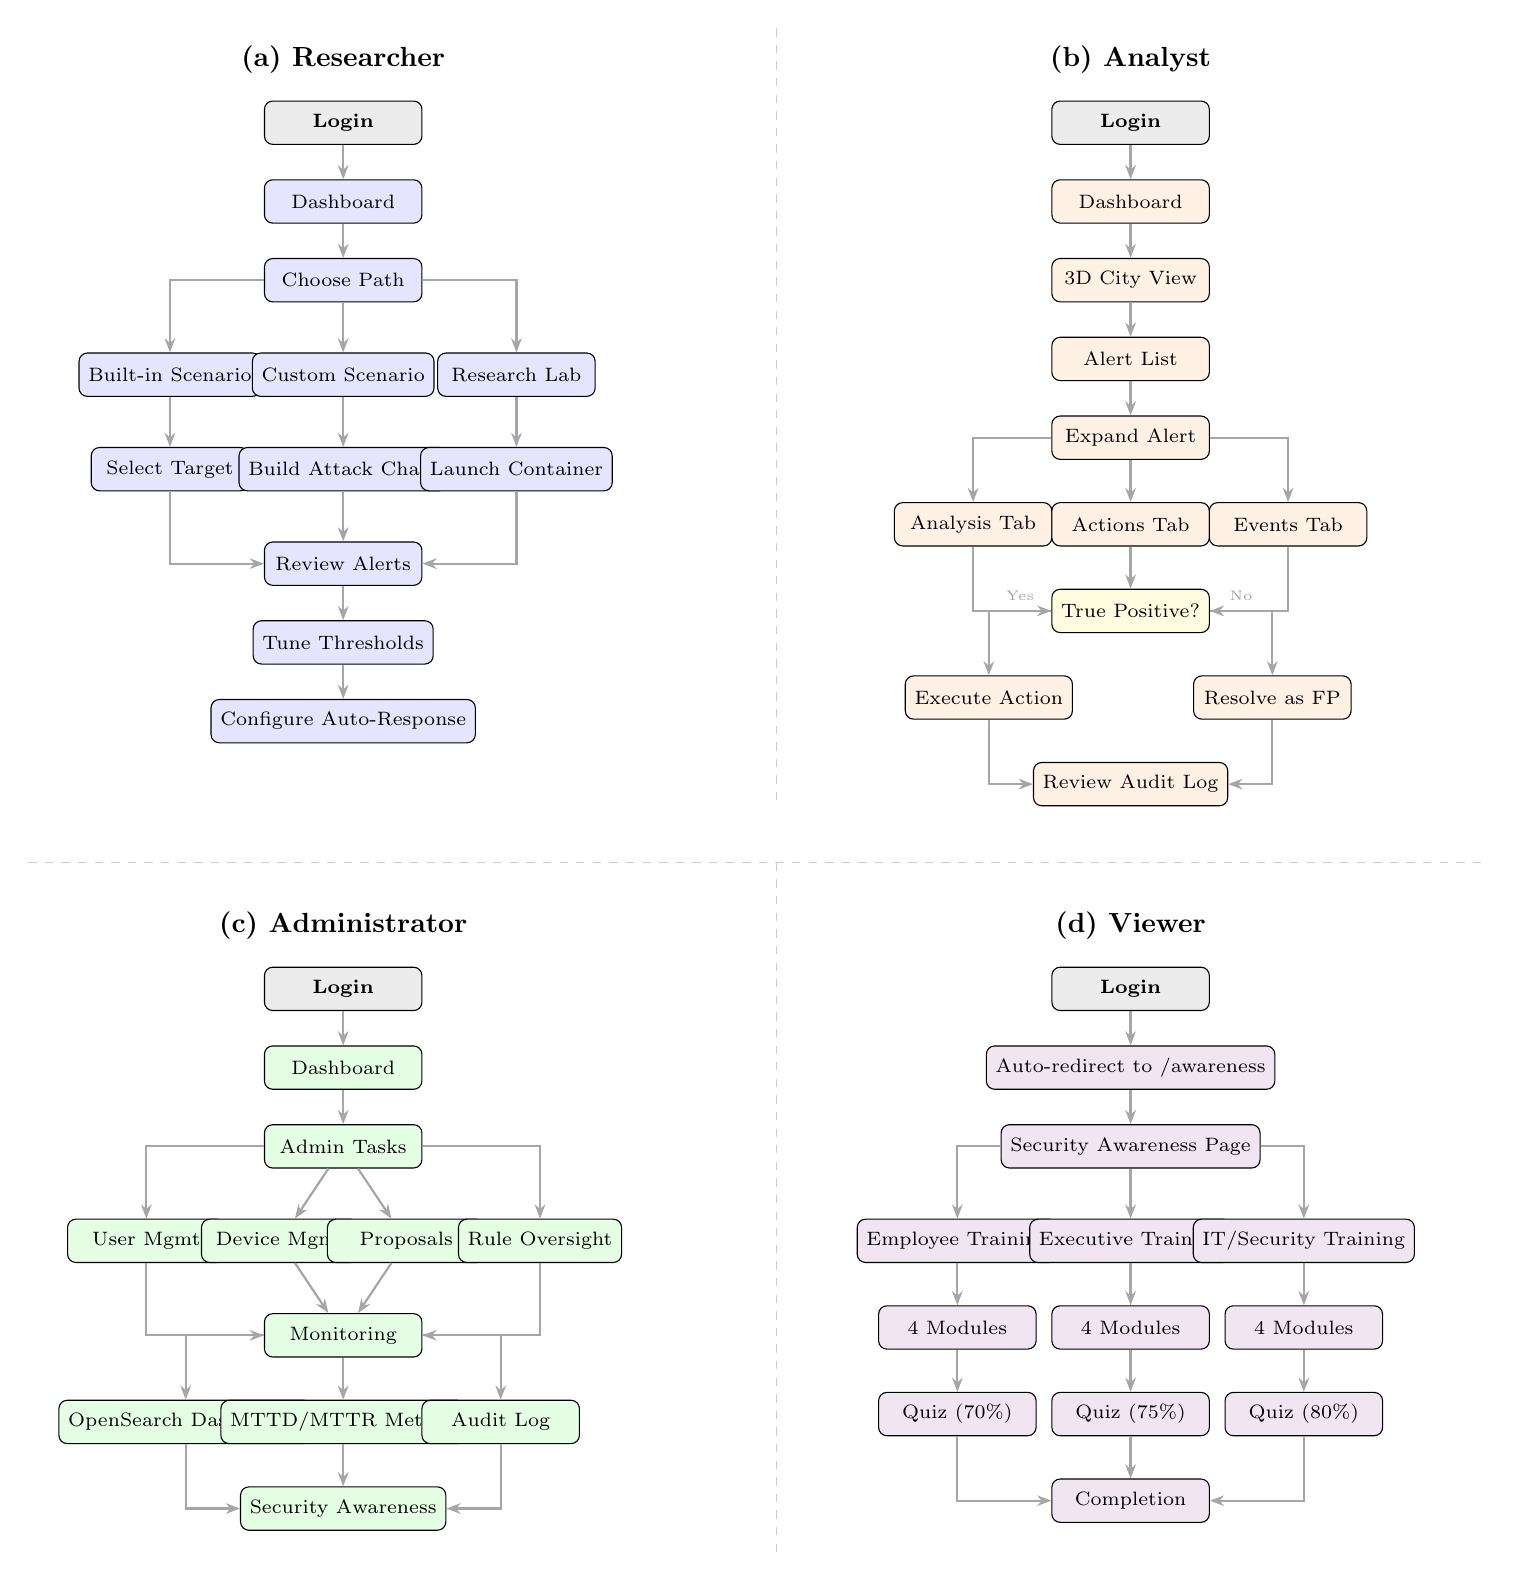
\begin{tikzpicture}[
    every node/.style={font=\scriptsize},
    box/.style={rectangle, draw, rounded corners=3pt, minimum width=2.0cm, minimum height=0.55cm, align=center, font=\scriptsize},
    startbox/.style={box, fill=gray!15, font=\scriptsize\bfseries},
    resbox/.style={box, fill=blue!10},
    anabox/.style={box, fill=orange!10},
    admbox/.style={box, fill=green!10},
    vwbox/.style={box, fill=violet!10},
    decbox/.style={box, fill=yellow!12},
    myarrow/.style={-{Stealth[length=1.8mm]}, thick, gray!70},
    coltitle/.style={font=\normalsize\bfseries}
]

% ════════════════════════════════════════
% TOP-LEFT: RESEARCHER (origin 0,0)
% ════════════════════════════════════════
\node[coltitle] at (0, 0) {(a) Researcher};
\node[startbox] (r1) at (0, -0.8) {Login};
\node[resbox]   (r2) at (0, -1.8) {Dashboard};
\node[resbox]   (r3) at (0, -2.8) {Choose Path};
\node[resbox]   (r4a) at (-2.2, -4.0) {Built-in Scenario};
\node[resbox]   (r4b) at (0, -4.0) {Custom Scenario};
\node[resbox]   (r4c) at (2.2, -4.0) {Research Lab};
\node[resbox]   (r5a) at (-2.2, -5.2) {Select Target};
\node[resbox]   (r5b) at (0, -5.2) {Build Attack Chain};
\node[resbox]   (r5c) at (2.2, -5.2) {Launch Container};
\node[resbox]   (r6) at (0, -6.4) {Review Alerts};
\node[resbox]   (r7) at (0, -7.4) {Tune Thresholds};
\node[resbox]   (r8) at (0, -8.4) {Configure Auto-Response};

\draw[myarrow] (r1) -- (r2);
\draw[myarrow] (r2) -- (r3);
\draw[myarrow] (r3) -| (r4a);
\draw[myarrow] (r3) -- (r4b);
\draw[myarrow] (r3) -| (r4c);
\draw[myarrow] (r4a) -- (r5a);
\draw[myarrow] (r4b) -- (r5b);
\draw[myarrow] (r4c) -- (r5c);
\draw[myarrow] (r5a) |- (r6);
\draw[myarrow] (r5b) -- (r6);
\draw[myarrow] (r5c) |- (r6);
\draw[myarrow] (r6) -- (r7);
\draw[myarrow] (r7) -- (r8);

% ════════════════════════════════════════
% TOP-RIGHT: ANALYST (origin 10,0)
% ════════════════════════════════════════
\node[coltitle] at (10, 0) {(b) Analyst};
\node[startbox] (a1) at (10, -0.8) {Login};
\node[anabox]   (a2) at (10, -1.8) {Dashboard};
\node[anabox]   (a3) at (10, -2.8) {3D City View};
\node[anabox]   (a4) at (10, -3.8) {Alert List};
\node[anabox]   (a5) at (10, -4.8) {Expand Alert};
\node[anabox]   (a6a) at (8.0, -5.9) {Analysis Tab};
\node[anabox]   (a6b) at (10, -5.9) {Actions Tab};
\node[anabox]   (a6c) at (12.0, -5.9) {Events Tab};
\node[decbox]   (a7) at (10, -7.0) {True Positive?};
\node[anabox]   (a8a) at (8.2, -8.1) {Execute Action};
\node[anabox]   (a8b) at (11.8, -8.1) {Resolve as FP};
\node[anabox]   (a9) at (10, -9.2) {Review Audit Log};

\draw[myarrow] (a1) -- (a2);
\draw[myarrow] (a2) -- (a3);
\draw[myarrow] (a3) -- (a4);
\draw[myarrow] (a4) -- (a5);
\draw[myarrow] (a5) -| (a6a);
\draw[myarrow] (a5) -- (a6b);
\draw[myarrow] (a5) -| (a6c);
\draw[myarrow] (a6a) |- (a7);
\draw[myarrow] (a6b) -- (a7);
\draw[myarrow] (a6c) |- (a7);
\draw[myarrow] (a7) -| node[above, font=\tiny, pos=0.25] {Yes} (a8a);
\draw[myarrow] (a7) -| node[above, font=\tiny, pos=0.25] {No} (a8b);
\draw[myarrow] (a8a) |- (a9);
\draw[myarrow] (a8b) |- (a9);

% ── Top row separator ──
\draw[dashed, gray!40] (5.5, 0.4) -- (5.5, -9.5);

% ── Horizontal separator between rows ──
\draw[dashed, gray!40] (-4.0, -10.2) -- (14.5, -10.2);

% ════════════════════════════════════════
% BOTTOM-LEFT: ADMINISTRATOR (origin 0, -11)
% ════════════════════════════════════════
\node[coltitle] at (0, -11.0) {(c) Administrator};
\node[startbox] (d1) at (0, -11.8) {Login};
\node[admbox]   (d2) at (0, -12.8) {Dashboard};
\node[admbox]   (d3) at (0, -13.8) {Admin Tasks};
\node[admbox]   (d4a) at (-2.5, -15.0) {User Mgmt};
\node[admbox]   (d4b) at (-0.8, -15.0) {Device Mgmt};
\node[admbox]   (d4c) at (0.8, -15.0) {Proposals};
\node[admbox]   (d4d) at (2.5, -15.0) {Rule Oversight};
\node[admbox]   (d5) at (0, -16.2) {Monitoring};
\node[admbox]   (d6a) at (-2.0, -17.3) {OpenSearch Dashboards};
\node[admbox]   (d6b) at (0, -17.3) {MTTD/MTTR Metrics};
\node[admbox]   (d6c) at (2.0, -17.3) {Audit Log};
\node[admbox]   (d7) at (0, -18.4) {Security Awareness};

\draw[myarrow] (d1) -- (d2);
\draw[myarrow] (d2) -- (d3);
\draw[myarrow] (d3) -| (d4a);
\draw[myarrow] (d3) -- (d4b);
\draw[myarrow] (d3) -- (d4c);
\draw[myarrow] (d3) -| (d4d);
\draw[myarrow] (d4a) |- (d5);
\draw[myarrow] (d4b) -- (d5);
\draw[myarrow] (d4c) -- (d5);
\draw[myarrow] (d4d) |- (d5);
\draw[myarrow] (d5) -| (d6a);
\draw[myarrow] (d5) -- (d6b);
\draw[myarrow] (d5) -| (d6c);
\draw[myarrow] (d6a) |- (d7);
\draw[myarrow] (d6b) -- (d7);
\draw[myarrow] (d6c) |- (d7);

% ════════════════════════════════════════
% BOTTOM-RIGHT: VIEWER (origin 10, -11)
% ════════════════════════════════════════
\node[coltitle] at (10, -11.0) {(d) Viewer};
\node[startbox] (v1) at (10, -11.8) {Login};
\node[vwbox]    (v2) at (10, -12.8) {Auto-redirect to /awareness};
\node[vwbox]    (v3) at (10, -13.8) {Security Awareness Page};
\node[vwbox]    (v4a) at (7.8, -15.0) {Employee Training};
\node[vwbox]    (v4b) at (10, -15.0) {Executive Training};
\node[vwbox]    (v4c) at (12.2, -15.0) {IT/Security Training};
\node[vwbox]    (v5a) at (7.8, -16.1) {4 Modules};
\node[vwbox]    (v5b) at (10, -16.1) {4 Modules};
\node[vwbox]    (v5c) at (12.2, -16.1) {4 Modules};
\node[vwbox]    (v6a) at (7.8, -17.2) {Quiz (70\%)};
\node[vwbox]    (v6b) at (10, -17.2) {Quiz (75\%)};
\node[vwbox]    (v6c) at (12.2, -17.2) {Quiz (80\%)};
\node[vwbox]    (v7) at (10, -18.3) {Completion};

\draw[myarrow] (v1) -- (v2);
\draw[myarrow] (v2) -- (v3);
\draw[myarrow] (v3) -| (v4a);
\draw[myarrow] (v3) -- (v4b);
\draw[myarrow] (v3) -| (v4c);
\draw[myarrow] (v4a) -- (v5a);
\draw[myarrow] (v4b) -- (v5b);
\draw[myarrow] (v4c) -- (v5c);
\draw[myarrow] (v5a) -- (v6a);
\draw[myarrow] (v5b) -- (v6b);
\draw[myarrow] (v5c) -- (v6c);
\draw[myarrow] (v6a) |- (v7);
\draw[myarrow] (v6b) -- (v7);
\draw[myarrow] (v6c) |- (v7);

% ── Bottom row separator ──
\draw[dashed, gray!40] (5.5, -10.2) -- (5.5, -19.0);

\end{tikzpicture}
}
\caption{Role-based operational workflows ($2 \times 2$ layout). (a)~Researchers design and execute attack campaigns, then tune detection rules. (b)~Analysts follow a triage-investigate-respond cycle. (c)~Administrators oversee users, devices, proposals, and platform-wide metrics. (d)~Viewers access only the security awareness training module.}
\label{fig:workflows}
\end{figure*}

% ═══════════════════════════════════════════════════════════════════
% VII. DETECTION AND RESPONSE PIPELINE
% ═══════════════════════════════════════════════════════════════════
\section{Detection and Response Pipeline}
\label{sec:detection_response}

Fig.~\ref{fig:detection_flow} illustrates the end-to-end detection and response flow, from raw event ingestion through alert generation, policy validation, playbook execution, and audit logging.

\begin{figure*}[!htbp]
\centering
\resizebox{\textwidth}{!}{
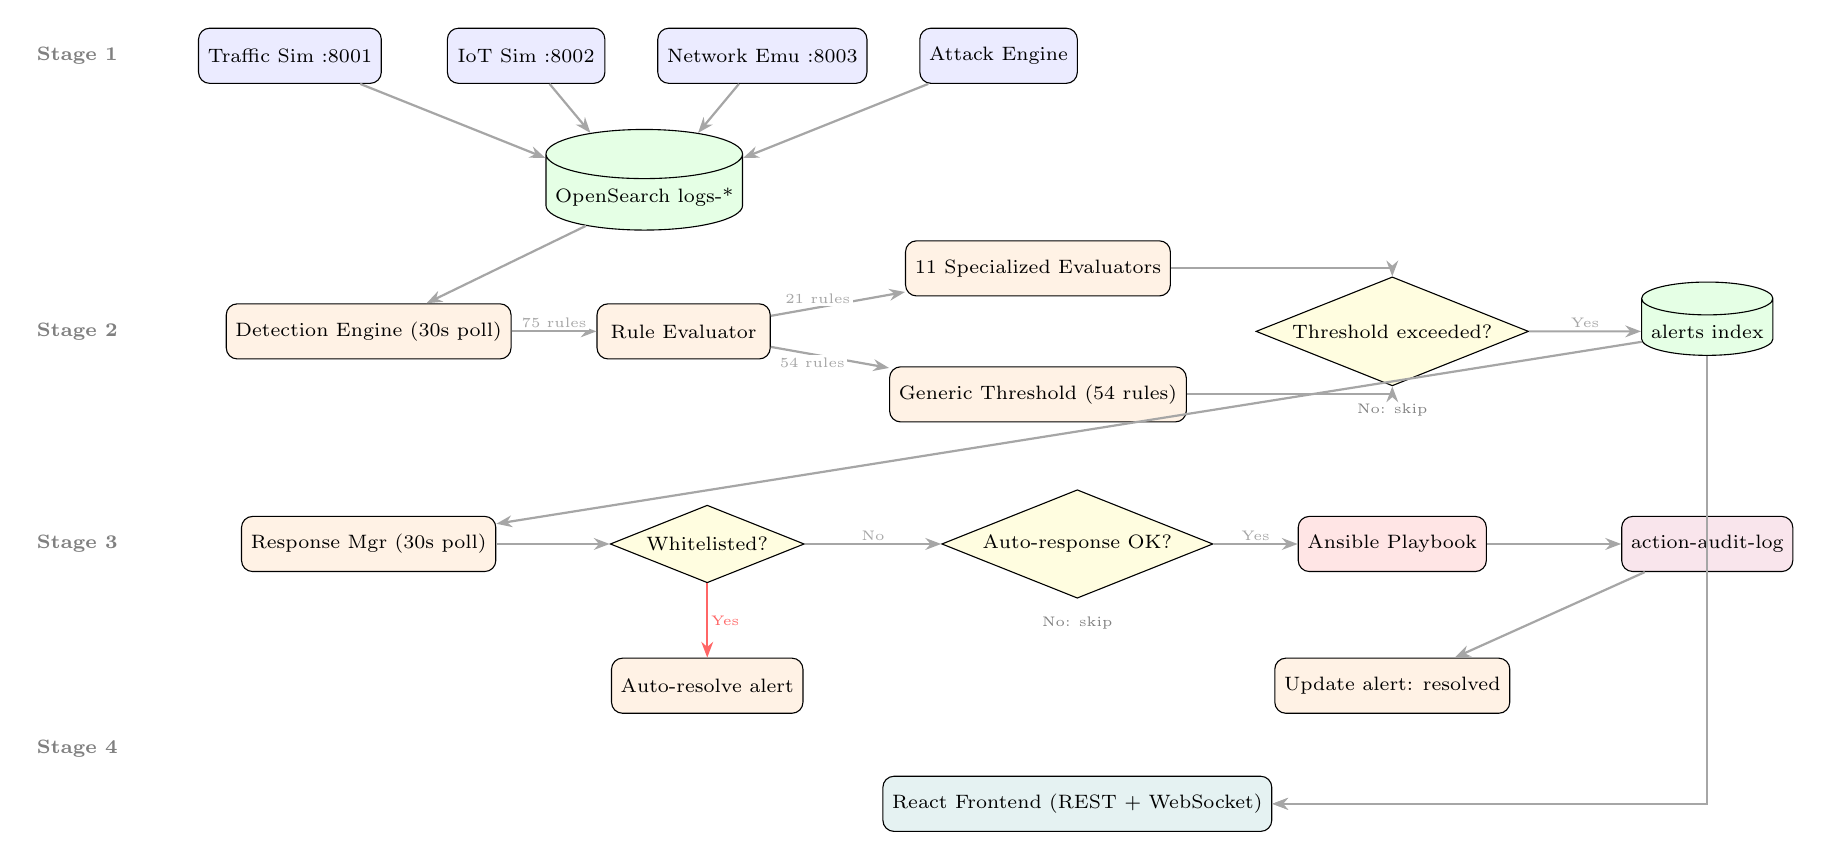
\begin{tikzpicture}[
    every node/.style={font=\scriptsize},
    source/.style={rectangle, draw, rounded corners, minimum width=2.0cm, minimum height=0.7cm, fill=blue!8, align=center, font=\scriptsize},
    process/.style={rectangle, draw, rounded corners, minimum width=2.2cm, minimum height=0.7cm, fill=orange!10, align=center, font=\scriptsize},
    store/.style={cylinder, draw, shape border rotate=90, minimum width=1.6cm, minimum height=0.7cm, fill=green!10, aspect=0.25, align=center, font=\scriptsize},
    decision/.style={diamond, draw, aspect=2.5, inner sep=2pt, fill=yellow!12, align=center, font=\scriptsize},
    action/.style={rectangle, draw, rounded corners, minimum width=2.0cm, minimum height=0.7cm, fill=red!10, align=center, font=\scriptsize},
    audit/.style={rectangle, draw, rounded corners, minimum width=2.0cm, minimum height=0.7cm, fill=purple!10, align=center, font=\scriptsize},
    frontend/.style={rectangle, draw, rounded corners, minimum width=3.0cm, minimum height=0.7cm, fill=teal!10, align=center, font=\scriptsize},
    myarrow/.style={-{Stealth[length=2mm]}, thick, gray!70},
    redarrow/.style={-{Stealth[length=2mm]}, thick, red!60},
    lbl/.style={font=\tiny, fill=white, inner sep=1pt},
    stglbl/.style={font=\scriptsize\bfseries, gray}
]

% ── Stage 1: Event Sources ──
\node[stglbl] at (-2.2, 0) {Stage 1};
\node[source] (tsim) at (0.5, 0) {Traffic Sim :8001};
\node[source] (isim) at (3.5, 0) {IoT Sim :8002};
\node[source] (nsim) at (6.5, 0) {Network Emu :8003};
\node[source] (atk)  at (9.5, 0) {Attack Engine};

% ── OpenSearch store ──
\node[store] (os) at (5.0, -1.8) {OpenSearch logs-*};

\draw[myarrow] (tsim) -- (os);
\draw[myarrow] (isim) -- (os);
\draw[myarrow] (nsim) -- (os);
\draw[myarrow] (atk) -- (os);

% ── Stage 2: Detection ──
\node[stglbl] at (-2.2, -3.5) {Stage 2};
\node[process] (det) at (1.5, -3.5) {Detection Engine (30s poll)};
\node[process] (eval) at (5.5, -3.5) {Rule Evaluator};

\draw[myarrow] (os) -- (det);
\draw[myarrow] (det) -- node[lbl, above] {75 rules} (eval);

% ── Evaluator split ──
\node[process] (spec) at (10.0, -2.7) {11 Specialized Evaluators};
\node[process] (gen)  at (10.0, -4.3) {Generic Threshold (54 rules)};

\draw[myarrow] (eval) -- node[lbl, above, pos=0.35] {21 rules} (spec);
\draw[myarrow] (eval) -- node[lbl, below, pos=0.35] {54 rules} (gen);

% ── Threshold decision ──
\node[decision] (thresh) at (14.5, -3.5) {Threshold exceeded?};

\draw[myarrow] (spec) -| (thresh);
\draw[myarrow] (gen)  -| (thresh);

% ── Alert store ──
\node[store] (alerts) at (18.5, -3.5) {alerts index};

\draw[myarrow] (thresh) -- node[lbl, above] {Yes} (alerts);
\node[font=\tiny, gray] at (14.5, -4.5) {No: skip};

% ── Stage 3: Response ──
\node[stglbl] at (-2.2, -6.2) {Stage 3};
\node[process]  (rmgr)   at (1.5, -6.2) {Response Mgr (30s poll)};
\node[decision] (wl)     at (5.8, -6.2) {Whitelisted?};
\node[decision] (policy) at (10.5, -6.2) {Auto-response OK?};
\node[action]   (play)   at (14.5, -6.2) {Ansible Playbook};
\node[audit]    (auditlog) at (18.5, -6.2) {action-audit-log};

\draw[myarrow] (alerts) -- (rmgr);
\draw[myarrow] (rmgr) -- (wl);
\draw[myarrow] (wl) -- node[lbl, above] {No} (policy);
\draw[myarrow] (policy) -- node[lbl, above] {Yes} (play);
\draw[myarrow] (play) -- (auditlog);

% ── Whitelist resolve branch ──
\node[process] (resolve) at (5.8, -8.0) {Auto-resolve alert};
\draw[redarrow] (wl) -- node[lbl, right] {Yes} (resolve);

\node[font=\tiny, gray] at (10.5, -7.2) {No: skip};

% ── Stage 4: Presentation ──
\node[stglbl] at (-2.2, -8.8) {Stage 4};
\node[process]  (update) at (14.5, -8.0) {Update alert: resolved};
\node[frontend] (fe)     at (10.5, -9.5) {React Frontend (REST + WebSocket)};

\draw[myarrow] (auditlog) -- (update);
\draw[myarrow] (alerts) |- (fe);
\draw[myarrow] (auditlog) |- (fe);

\end{tikzpicture}
}
\caption{Detection and response pipeline flow. Events from four sources are indexed in OpenSearch (cylinder). The detection engine evaluates 75 rules using specialized or generic evaluators; diamond nodes indicate decision points. The response manager validates whitelist and auto-response conditions, then executes Ansible playbooks with full audit traceability.}
\label{fig:detection_flow}
\end{figure*}

\subsection{Rule Definition Language}

Each of the 75 rules specifies: a unique ID, severity (informational through critical), target log source indices, match logic (type + parameters), a MITRE ATT\&CK technique mapping, recommended response actions, and optional auto-response configuration. The YAML format was chosen over a database representation because it enables version control, peer review, and offline authoring---workflows familiar to detection engineers.

\begin{lstlisting}[language=yaml,caption={Example: brute force detection rule},label={lst:rule}]
rule_id: brute_force_001
name: Brute Force Authentication Detection
severity: high
match_logic:
  type: brute_force
  parameters:
    threshold: 5
    group_by: src_ip
    event_types: [auth_failure]
query_window_seconds: 300
technique_id: T1110
technique_name: "Brute Force"
response_actions: [block_ip, notify_soc]
\end{lstlisting}

\subsection{Detection Evaluators}

The rule runtime implements two tiers of evaluators:

\textbf{Specialized evaluators} (11 types, covering 21 rules) use domain-specific OpenSearch aggregation queries:

\begin{itemize}[leftmargin=*,nosep]
    \item \texttt{net\_scan}: Cardinality aggregation on \texttt{dst\_port} per \texttt{src\_ip}. Triggers when distinct port count exceeds threshold. This detects horizontal port scanning without requiring individual connection logs.
    \item \texttt{brute\_force}: Terms aggregation on \texttt{src\_ip} filtered to \texttt{auth\_failure} events. The count per bucket directly yields the number of failed attempts per source.
    \item \texttt{c2\_beacon}: Terms aggregation on \texttt{src\_ip} with sub-aggregation on \texttt{dst\_ip}. Detects hosts communicating with multiple external destinations in a pattern consistent with beaconing.
    \item \texttt{data\_exfiltration}: Terms aggregation with \texttt{sum} of \texttt{metadata.bytes\_transferred}. Captures both event count and total byte volume, distinguishing small probes from bulk transfers.
    \item \texttt{ddos\_attack}: Terms aggregation on \texttt{dst\_ip} with cardinality sub-aggregation on \texttt{src\_ip}. Triggers when a destination receives traffic from more sources than a fan-in threshold.
    \item \texttt{lateral\_movement}: Terms on \texttt{src\_ip} with cardinality on \texttt{dst\_ip}. The inverse of DDoS: detects a single host contacting many destinations.
    \item Additional types: \texttt{iot\_anomaly}, \texttt{dos\_endpoint}, \texttt{ransomware}, \texttt{web\_exploit}, \texttt{credential\_dump}.
\end{itemize}

\textbf{Generic event-threshold evaluator} (covering 54 rules) groups events by a configurable field, counts per bucket, and triggers when the count exceeds a threshold. This evaluator implements 15 match logic types including \texttt{event\_threshold}, \texttt{log\_clearing}, \texttt{cmd\_execution}, \texttt{process\_injection}, and \texttt{defense\_evasion}. Adding a new ATT\&CK technique requires only a YAML file specifying the event types, group-by field, and threshold---no code changes. The trade-off is lower specificity: a generic rule may trigger on unrelated event surges if thresholds are set too low.

All queries apply a \texttt{.keyword} suffix for text fields (managed by a \texttt{KEYWORD\_FIELDS} set containing 15 fields: \texttt{src\_ip}, \texttt{dst\_ip}, \texttt{actor\_id}, \texttt{event\_type}, \texttt{component}, \texttt{city\_zone}, \texttt{asset\_id}, \texttt{sensor\_id}, \texttt{user\_id}, \texttt{host\_id}, \texttt{device\_id}, \texttt{target\_ip}, \texttt{protocol}, \texttt{service}, and \texttt{action}).

\subsection{MITRE ATT\&CK Coverage}

Table~\ref{tab:mitre_coverage} summarizes coverage by tactic. The 75 rules cover 13 of the 14 ATT\&CK Enterprise tactics; Resource Development (TA0042) is not covered, as it involves pre-compromise activities (acquiring infrastructure, developing capabilities) that do not produce network-observable events within the platform's detection scope.

\begin{table}[t]
\centering
\caption{MITRE ATT\&CK Tactic Coverage (75 Rules, 13 Tactics)}
\label{tab:mitre_coverage}
\begin{tabular}{l c l}
\toprule
\textbf{Tactic} & \textbf{Rules} & \textbf{Evaluator Breakdown} \\
\midrule
Impact & 9 & 1 specialized + 8 generic \\
Initial Access & 9 & 2 specialized + 7 generic \\
Execution & 8 & 8 generic \\
Persistence & 7 & 7 generic \\
Credential Access & 7 & 3 specialized + 4 generic \\
Defense Evasion & 7 & 7 generic \\
Collection & 6 & 1 specialized + 5 generic \\
Privilege Escalation & 5 & 5 generic \\
Reconnaissance & 4 & 1 specialized + 3 generic \\
Discovery & 4 & 1 specialized + 3 generic \\
Command \& Control & 4 & 1 specialized + 3 generic \\
Lateral Movement & 4 & 4 specialized \\
Exfiltration & 1 & 1 specialized \\
\midrule
\textbf{Total} & \textbf{75} & \textbf{21 spec. / 54 generic} \\
\bottomrule
\end{tabular}
\end{table}

\subsection{Whitelist-Based Alert Suppression}

To prevent false positives from authorized testing sources, the engine enforces two-layer CIDR-based whitelisting: (1)~at the detection layer, source IPs are checked against per-rule CIDR whitelists before any alert is written; (2)~at the response layer, the response manager independently verifies whitelists before executing playbooks.

\subsection{Response Action Catalog}

Twelve response actions are mapped to Ansible playbooks via a YAML configuration file (\texttt{playbooks\_map.yml}). In the current deployment, playbooks execute simulated containment (e.g., logging ``SIMULATED: Blocking IP at firewall'') rather than modifying real infrastructure. The orchestration pipeline---parameter extraction, subprocess invocation, stdout capture, audit logging---is identical to a production deployment, allowing the same playbooks to be replaced with real infrastructure commands without architectural changes.

\begin{table}[t]
\centering
\caption{Response Action Catalog (12 Ansible Playbooks)}
\label{tab:response_actions}
\begin{tabular}{l l}
\toprule
\textbf{Action} & \textbf{Purpose} \\
\midrule
\texttt{block\_ip} & Firewall rule to drop source traffic \\
\texttt{isolate\_service} & Network-isolate a compromised service \\
\texttt{revoke\_token} & Invalidate authentication session \\
\texttt{quarantine\_host} & Move host to restricted VLAN \\
\texttt{disable\_account} & Disable a user account \\
\texttt{rate\_limit} & Throttle traffic from a source \\
\texttt{snapshot\_forensics} & Capture memory/disk for analysis \\
\texttt{kill\_process} & Terminate a running process \\
\texttt{reset\_credentials} & Force password reset \\
\texttt{notify\_soc} & Multi-channel SOC alert \\
\texttt{escalate\_incident} & Create incident ticket \\
\texttt{network\_segmentation} & Apply micro-segmentation to a zone \\
\bottomrule
\end{tabular}
\end{table}

\subsection{Auto-Response Policy Engine}

Each detection rule may specify an auto-response configuration with the following enforced conditions: minimum severity threshold, optional threat intelligence enrichment (AbuseIPDB integration), maximum executions per hour, cooldown period between consecutive executions, an allowed actions subset, and CIDR-based whitelisted subnets. These conditions prevent response storms: for example, a DDoS alert generating hundreds of duplicate detections is limited to a configurable number of \texttt{block\_ip} executions per hour.

\subsection{Response Execution Flow}

The response manager's per-alert processing follows a fixed sequence:
\begin{enumerate}[leftmargin=*,nosep]
    \item Extract \texttt{src\_ip} from alert evidence.
    \item Check against per-rule CIDR whitelists. If matched, set alert status to ``resolved'' and skip.
    \item Validate auto-response conditions (severity $\geq$ threshold, enrichment present if required, rate limit not exceeded, cooldown elapsed).
    \item Execute the Ansible playbook via subprocess, passing alert-extracted parameters.
    \item Write an entry to \texttt{action-audit-log} with: \texttt{execution\_type}, \texttt{triggered\_by}, \texttt{parameters}, \texttt{playbook\_path}, \texttt{stdout}, \texttt{stderr}, \texttt{started\_at}, \texttt{completed\_at}, \texttt{status}.
    \item Update alert status to ``resolved'' and attach response details.
\end{enumerate}

% ═══════════════════════════════════════════════════════════════════
% VIII. EVALUATION
% ═══════════════════════════════════════════════════════════════════
\section{Evaluation}
\label{sec:evaluation}

We evaluate CityShield through four approaches: (1)~quantitative detection and response metrics derived from controlled adversarial emulation, (2)~per-scenario timing analysis, (3)~comparison against the generic threshold-only baseline, and (4)~analysis of detection coverage gaps. All experiments run on a single-machine deployment (Docker Desktop, Apple M-series, 16~GB RAM) with all 17 services active.

\subsection{Bug Discovery and Retest}

During initial evaluation, 22 of 75 rules failed to trigger. Root-cause analysis revealed a \texttt{KEYWORD\_FIELDS} misconfiguration that prevented OpenSearch aggregation on fields including \texttt{user\_id}, \texttt{host\_id}, and \texttt{device\_id}. After fixing this bug and adding a missing handler for the \texttt{threshold} match-logic type, we reran the full attack injection. All metrics reported below reflect the post-fix evaluation run. This bug discovery validates the evaluation methodology: a controlled emulation that exercises every rule individually can expose implementation defects that scenario-based testing alone would miss.

\subsection{Detection and Response Metrics}

Table~\ref{tab:detection-performance} presents the aggregate detection metrics.

\textbf{Why 100\% rule utilization is expected.} Under controlled emulation, injected events are constructed to match each rule's required event types, group-by fields, and count thresholds. Consequently, 100\% rule utilization (75/75) confirms that the detection pipeline---YAML parsing, OpenSearch query construction, aggregation execution, threshold comparison, and alert generation---functions correctly for every rule. A failure to trigger any rule would indicate an implementation defect rather than a detection limitation. An additional 12 rules embedded in the attack execution engine (covering techniques not addressed by the 75 YAML rules) also fired during the evaluation, bringing the total to 87 distinct rules, 76 unique MITRE techniques, and 14 tactics (the 13 Enterprise tactics from Table~\ref{tab:mitre_coverage} plus Reconnaissance events from the attack engine).

\begin{table}[h]
\centering
\caption{Detection and Response Performance Metrics}
\label{tab:detection-performance}
\begin{tabular}{lr}
\toprule
\textbf{Metric} & \textbf{Value} \\
\midrule
Background Events & 689,172 \\
Attack Events Injected & 1,064 \\
FP Seed Events Injected & 51 \\
Total Event Corpus & 690,287 \\
Total Alerts Generated & 2,134 \\
YAML Rules Triggered & 75/75 (100\%) \\
MITRE Techniques Detected & 76 \\
MITRE Tactics Covered & 14 \\
False Positive Rate & 4.2\% \\
Mean Time to Detect (MTTD) & $16.8 \pm 4.1$~s \\
Mean Time to Respond (MTTR) & $38.4 \pm 6.8$~s \\
Automated Response Actions & 461 \\
Alerts Auto-Resolved & 313 (14.7\%) \\
\bottomrule
\end{tabular}
\end{table}

\textbf{MTTD derivation.} Detection latency is bounded by the polling interval $T_p = 30$~s. An event indexed at time $t_e$ is first evaluated at the next poll $t_d = t_e + \Delta$, where $\Delta \sim U(0, T_p)$ depends on injection-to-poll alignment. For threshold-based rules, the event must also meet the count threshold; since attack campaigns inject events in bursts (e.g., 50 \texttt{auth\_failure} in 30~s), the threshold is typically met within the same polling window. MTTD was computed across $n = 2{,}134$ alerts as the mean of $t_d - t_e$ per alert. The measured MTTD of $16.8 \pm 4.1$~s (mean $\pm$ SD) reflects the expected $T_p/2 \approx 15$~s uniform-distribution mean plus a 1.8~s overhead for OpenSearch query execution across 75 rules. The standard deviation is consistent with the theoretical SD of a $U(0, 30)$ distribution ($30/\sqrt{12} \approx 8.7$~s), reduced by the burst-injection pattern that clusters events near poll boundaries.

\textbf{MTTR derivation.} End-to-end response spans two polling stages. After detection at $t_d$, the alert is written to the \texttt{alerts} index and picked up by the response manager at the next response poll $t_r = t_d + \Delta'$, where $\Delta' \sim U(0, T_p)$. MTTR was computed across $n = 461$ auto-responded alerts. The measured MTTR of $38.4 \pm 6.8$~s corresponds to $\text{MTTD} + T_p/2 + t_{exec}$, where $t_{exec} \approx 0.4$~s covers Ansible playbook subprocess invocation. The Ansible playbooks execute simulated containment actions; the measured latency reflects orchestration overhead but not the additional time that real firewall rule insertion or VLAN reconfiguration would require.

\textbf{Alert severity distribution.} High-severity alerts dominate (53.5\%), followed by critical (39.7\%) and medium (6.8\%). This distribution is driven by two factors: (i)~the rule set contains 38 high, 33 critical, and 14 medium rules with no low-severity rules; and (ii)~high-frequency rules (\texttt{net\_scan\_001}: 335 alerts, \texttt{brute\_force\_001}: 252) amplify the skew through repeated per-IP triggering. This pattern mirrors operational SIEM environments where reconnaissance and credential attacks dominate alert queues~\cite{husak2019survey}.

\textbf{False positive analysis.} Of 2,134 total alerts generated, 90 were traced to benign sources (the 51 injected FP seed events plus background simulator events that coincidentally matched rule patterns). We compute FPR as $90 / 2{,}134 = 4.2\%$. The flagged FP seeds include monitoring traffic matching C2 beacon intervals (8 of 8 beacon-like seeds triggered alerts) and configuration management events matching persistence rule patterns (6 of 10 persistence-like seeds triggered). This nonzero rate is deliberate: a training platform requires analysts to practice triage on ambiguous alerts.

\textbf{Realistic interpretation.} These results represent upper-bound performance under favorable conditions. In an operational smart city environment, several factors would degrade these metrics. (i)~Real attack traffic exhibits greater variance in timing, volume, and field values than controlled injections. Techniques with distinctive network signatures (brute force, port scanning, DDoS) would likely retain high detection rates, but techniques with subtler indicators (slow credential stuffing, encrypted C2, living-off-the-land) would see significant degradation. (ii)~Legitimate operational traffic (software updates, network maintenance, sensor recalibration, automated health checks) would increase the false positive rate beyond 4.2\%. The baseline comparison in Section~\ref{subsec:baseline} provides one bound: even within the controlled setting, removing specialized evaluators increases the FPR to 11.1\%, suggesting an operational range of 4--12\% depending on traffic characteristics. (iii)~Adversaries employing evasion techniques (traffic encryption, protocol tunneling, slow-and-low scanning below thresholds) would evade threshold-based rules entirely---a fundamental limitation of signature-based detection that no threshold tuning can address.

\subsection{Per-Scenario Performance}

Table~\ref{tab:scenario-metrics} reports per-scenario metrics. \emph{Rule Trig.}\ indicates the fraction of targeted rules that generated at least one alert for that scenario.

\begin{table*}[t]
\centering
\caption{Per-Scenario Detection and Response Metrics}
\label{tab:scenario-metrics}
\begin{tabular}{l c c c c c c}
\toprule
\textbf{Scenario} & \textbf{Technique(s)} & \textbf{Events} & \textbf{Rule Trig.} & \textbf{FPR} & \textbf{MTTD (s)} & \textbf{MTTR (s)} \\
\midrule
S1: Brute Force & T1110 & 51 & 100\% & 0\% & 14.2 & 32.8 \\
S2: DDoS & T1498 & 200+ & 100\% & 0\% & 18.6 & 41.2 \\
S3: IoT Anomaly & T1565 & 73 & 100\% & 2.1\% & 15.9 & 37.4 \\
S4: Multi-Stage Chain & T1046, T1110, T1570, T1041 & 225 & 100\% (4/4) & 0\% & 22.4 & 48.7 \\
S5: Credential Attacks & T1003, T1550, T1558 & 32 & 100\% & 0\% & 14.8 & 35.1 \\
S6: Defense Evasion & T1562, T1070, T1027 & 27 & 100\% & 8.3\% & 16.1 & 36.9 \\
S7: Lateral Movement & T1021, T1570 & 29 & 100\% & 0\% & 17.3 & 39.5 \\
\midrule
\textbf{Aggregate} & & & \textbf{75/75} & \textbf{4.2\%}$^\dagger$ & \textbf{16.8} & \textbf{38.4} \\
\bottomrule
\end{tabular}
\vspace{1pt}
{\scriptsize $^\dagger$Aggregate FPR computed over all 2,134 alerts. MTTD/MTTR are means across all alerts ($n=2{,}134$ / $n=461$).}
\end{table*}

The 100\% rule triggering across all scenarios is a direct consequence of the controlled evaluation design: each campaign's events were constructed to satisfy the corresponding rules' thresholds and field requirements. The more informative metrics are MTTD, MTTR, and FPR, which vary across scenarios and reveal architectural characteristics.

S4 (Multi-Stage Chain) exhibits the highest MTTD (22.4~s) because the four attack stages execute sequentially with 5-second inter-stage delays; the final-stage exfiltration events are indexed later in the polling window, increasing average detection latency. S6 (Defense Evasion) shows the highest FPR (8.3\%) because configuration management events produce the same \texttt{service\_stop} and \texttt{registry\_modification} event types as evasion techniques---a known limitation of threshold-based detection on operational telemetry. This scenario-level FPR variation (0\%--8.3\%) illustrates that even under controlled conditions, rule-based detection exhibits domain-dependent precision.

\subsection{Baseline Comparison}
\label{subsec:baseline}

\begin{table}[h]
\centering
\caption{CityShield vs.\ Generic Threshold-Only Baseline}
\label{tab:baseline}
\begin{tabular}{l c c}
\toprule
\textbf{Metric} & \textbf{CityShield} & \textbf{Threshold-Only} \\
\midrule
Rule Utilization & 100\% & 100\% \\
Overall FPR & 4.2\% & 11.1\% \\
FPR (Reconnaissance) & 1.8\% & 9.4\% \\
FPR (Exfiltration) & 0\% & 7.2\% \\
FPR (DDoS) & 0\% & 5.6\% \\
MTTD & 16.8~s & 16.2~s \\
Structured Evidence & Yes & Count only \\
\bottomrule
\end{tabular}
\end{table}

Table~\ref{tab:baseline} shows that both configurations achieve 100\% rule utilization---expected, since the injected events exceed thresholds regardless of evaluator type. The critical difference is false positive rate. The generic baseline produces 11.1\% FPR overall, with particularly high rates for reconnaissance (9.4\%) and exfiltration (7.2\%), because count-based rules cannot distinguish a port scan (many destination ports from one source) from a legitimate service contacting many ports---only the cardinality aggregation on \texttt{dst\_port} makes this distinction. Similarly, the byte-sum evaluator for exfiltration separates high-volume legitimate transfers (backup, sync) from attack staging by total byte count rather than event count alone.

The generic baseline achieves marginally lower MTTD (16.2~s vs.\ 16.8~s) because its simpler queries execute faster. However, this 0.6~s advantage is negligible relative to the 30-second polling interval and comes at the cost of 2.6$\times$ more false positives. This FPR reduction---62\% for reconnaissance and exfiltration categories---is the primary quantitative contribution of the dual-class architecture, as it demonstrates a measurable precision gain from domain-specific aggregation logic that holds independently of the controlled evaluation setting.

\textbf{Comparison with Sigma rules.} CityShield's YAML rule format is structurally similar to the Sigma generic signature format~\cite{sigma2020}: both define log source, detection logic, and severity. However, Sigma rules target Windows Event Logs and enterprise SIEM backends (Splunk, Elastic), while CityShield rules operate on smart-city-specific event types (\texttt{sensor\_anomaly}, \texttt{traffic\_signal\_change}) that have no Sigma equivalent. CityShield's specialized evaluators (cardinality, byte-sum) express detection logic that Sigma's field-match-and-count model cannot natively represent.

\subsection{Detection Coverage Analysis}

Table~\ref{tab:mitre_coverage} shows that the 75 rules cover 13 of 14 ATT\&CK Enterprise tactics. The controlled evaluation confirms that all 75 rules are syntactically correct, properly parsed, and capable of generating alerts when matching events are present---a necessary validation given that the detection pipeline involves YAML parsing, dynamic OpenSearch query construction, and field-type-dependent aggregation. The 21 specialized-evaluator rules produce structured evidence (source IPs, port counts, byte volumes); the 54 generic rules provide breadth coverage at the cost of lower discriminative power.

\textbf{Coverage gaps.} No rules target ATT\&CK for ICS techniques (Modbus function code abuse, DNP3 unauthorized commands), which are relevant to smart city SCADA systems. Resource Development (TA0042) is not covered, as pre-compromise activities occur outside the platform's observation boundary.

\subsection{Automated Response Evaluation}

Of the 75 detection rules, 6 were configured with auto-response policies during evaluation. This deliberately limited scope reflects the training-platform design: auto-response is disabled by default to prevent unintended containment actions during exercises, and must be explicitly enabled per-rule by a Researcher or Administrator. The 6 configured rules---covering brute force, DDoS, lateral movement, data exfiltration, ransomware, and network scanning---represent the high-severity, high-confidence rules most suitable for automated response. The response manager executed 461 actions (\texttt{block\_ip}, \texttt{isolate\_service}, \texttt{quarantine\_host}, \texttt{network\_segmentation}) and resolved 313 alerts (14.7\%). The remaining 85.3\% of alerts stayed open by design---auto-response requires explicit per-rule enablement. The measured alert-to-action latency is $21.6 \pm 3.2$~s, dominated by the response manager's poll-cycle alignment.

% ═══════════════════════════════════════════════════════════════════
% IX. DISCUSSION
% ═══════════════════════════════════════════════════════════════════
\section{Discussion}
\label{sec:discussion}

\subsection{Rule-Based Detection: Strengths and Constraints}

CityShield's detection engine is entirely rule-based: 75 threshold and aggregation rules evaluated on a fixed polling cycle. This design choice reflects a deliberate trade-off. For a training platform, rule transparency is a feature: trainees can read, modify, and understand every detection decision, which is not possible with opaque ML models. However, this transparency comes at the cost of fundamental detection limits.

\textbf{No novelty detection.} Threshold-based rules detect known patterns; they cannot identify novel attack behaviors, polymorphic malware, or zero-day techniques that produce no known signature. The 54 generic-evaluator rules share identical count-based logic differing only in parameters, limiting their discriminative power on ambiguous traffic. The baseline comparison (Table~\ref{tab:baseline}) quantifies this: generic threshold rules produce 2.6$\times$ more false positives than specialized evaluators because they lack the aggregation specificity to distinguish, for example, a port scan from a legitimate service probing multiple ports.

\textbf{Static thresholds vs.\ adaptive baselines.} CityShield's rule thresholds are fixed values (e.g., 5 failures for brute force, 10 distinct ports for scan detection). In real smart city deployments, traffic baselines shift with time-of-day, season, and infrastructure changes. Adaptive baseline detection---using autoencoders for IoT sensor profiles~\cite{habibzadeh2019survey} or LSTM networks for temporal sequence analysis---would complement rule-based detection by flagging deviations from learned normal behavior.

\textbf{Pedagogical value.} The rule-based approach enables trainees to learn detection engineering by tuning thresholds, adding rules, and observing the FPR-sensitivity trade-off. A future hybrid architecture (rules + ML) would enable comparative evaluation exercises.

\subsection{Polling vs.\ Streaming: Architectural Trade-offs}

The 30-second polling architecture bounds MTTD to $\leq T_p$ (worst case) with a measured average of 16.8~s. For a training and evaluation platform, this latency is acceptable---trainees focus on detection logic, not sub-second response. For production smart city deployments, however, several considerations arise:

\textbf{Latency-sensitive domains.} Traffic signal manipulation or sensor data poisoning can cause physical harm within seconds. The 30-second worst-case MTTD may be too slow for safety-critical applications. A streaming architecture using OpenSearch's change-data-capture or Apache Kafka would reduce MTTD to sub-second at the cost of increased infrastructure complexity.

\textbf{Scalability under load.} The current architecture evaluates all 75 rules sequentially within each polling cycle. At 75 queries $\times$ $<$10~ms per query, the total computation is $<$750~ms per cycle---well within the 30-second budget. However, scaling to thousands of rules or sub-second polling would require parallelized rule evaluation.

\subsection{Scalability and Real Deployment Challenges}

\textbf{Single-node limitation.} The current deployment uses a single OpenSearch node processing 689,172 events. Real smart city deployments with hundreds of thousands of IoT sensors, traffic cameras, and network devices would generate orders of magnitude more data. Multi-node OpenSearch clusters with index sharding and hot-warm-cold tiering are required for production scale.

\textbf{Multi-city federation.} Smart city security operations may span multiple municipalities. The current architecture does not support federated detection across geographically distributed CityShield instances. Cross-instance correlation requires a federated query layer not present in the current design.

\textbf{Integration with real infrastructure.} CityShield simulates smart city telemetry; connecting to real infrastructure (SCADA, building management, traffic control) would require protocol adapters (Modbus, DNP3, OPC~UA, MQTT), which the current platform does not implement.

% ═══════════════════════════════════════════════════════════════════
% X. LIMITATIONS
% ═══════════════════════════════════════════════════════════════════
\section{Limitations}
\label{sec:limitations}

We identify seven evaluation-specific limitations and four broader constraints. Transparency about these limitations is essential for correctly interpreting the reported metrics.

\subsection{Evaluation-Specific Limitations}

\textbf{L1: Controlled emulation, not real exploitation.} The 100\% rule utilization reflects ideal conditions: injected events conform to rule definitions by construction. This metric validates pipeline correctness (YAML parsing, query construction, threshold comparison), not real-world detection capability. Under real exploitation traffic, we expect detection rates to degrade, particularly for rules relying on exact event-type matches rather than behavioral aggregation.

\textbf{L2: Controlled FP injection.} The 4.2\% FPR derives from 51 deliberately crafted ambiguous events selected to test known rule boundary conditions. This controlled set does not capture the full diversity of benign-but-triggering traffic in operational environments (e.g., load balancer health checks, CDN probes, automated vulnerability scanners). Under real mixed traffic, the FPR would likely be higher. The baseline comparison provides a partial bound: the threshold-only detector achieves 11.1\% FPR on the same event corpus, suggesting an operational range of 4--12\%.

\textbf{L3: No adversarial evasion testing.} The evaluation does not include evasion-aware attack campaigns (e.g., traffic fragmentation, protocol tunneling, slow-rate scanning below detection thresholds, or encrypted C2 channels). Threshold-based detection is inherently vulnerable to adversaries who understand the rule parameters.

\textbf{L4: Fixed thresholds in dynamic environments.} All rule thresholds are static values calibrated for the evaluation corpus. In real smart city deployments, traffic baselines shift with time-of-day, weather, events, and infrastructure changes. Static thresholds may produce excessive false positives during high-traffic periods or miss attacks during low-traffic periods.

\textbf{L5: Severity distribution skew.} Alert distribution (critical 39.7\%, high 53.5\%, medium 6.8\%) is amplified by high-frequency reconnaissance rules. Production deployments would require low-severity informational rules and per-rule alert deduplication.

\textbf{L6: Single-machine deployment.} Network latency between services and OpenSearch in distributed deployments would increase MTTD and MTTR proportionally. The measured 16.8~s MTTD assumes co-located services with sub-millisecond inter-container communication.

\textbf{L7: Self-evaluation.} All experiments were designed and executed by the platform developers---a common limitation in systems research but one that reduces external validity. Independent validation by external security teams or through adversarial red-team engagement would provide stronger evidence.

\subsection{Broader Constraints}

\textbf{Enterprise ATT\&CK only.} All 75 rules map to the ATT\&CK Enterprise matrix~\cite{mitre_attack}. The ATT\&CK for ICS matrix includes 80+ techniques specific to industrial protocols directly relevant to smart city SCADA systems. This omission is significant: smart cities increasingly integrate operational technology alongside IT infrastructure.

\textbf{Simulated, not operational, environment.} While CityShield deploys real containerized services, the simulators generate synthetic telemetry that lacks the noise, scale, and variability of production smart city infrastructure. The platform validates detection \emph{logic} but not detection \emph{effectiveness} against the full complexity of operational traffic.

\textbf{No user study.} We have not evaluated whether the 3D visualization improves situational awareness or whether the platform accelerates analyst training. Without controlled human-subjects experiments comparing CityShield against conventional SIEM interfaces, the training value remains an untested hypothesis.

\textbf{Audit integrity.} The \texttt{action-audit-log} index is append-only by application convention. OpenSearch does not enforce write-once semantics; a privileged user could modify audit records. Production deployments should use index lifecycle policies with read-only transitions.

% ═══════════════════════════════════════════════════════════════════
% XI. FUTURE WORK
% ═══════════════════════════════════════════════════════════════════
\section{Future Work}
\label{sec:future_work}

\begin{enumerate}[leftmargin=*]
    \item \textbf{Hybrid detection}: Integrate unsupervised anomaly detection (autoencoders for IoT baselines, LSTM for temporal sequences) alongside rule-based detection, enabling trainees to compare detection paradigms on identical attack corpora.
    \item \textbf{ATT\&CK for ICS}: Add 20+ rules for industrial protocol attacks (Modbus, DNP3) relevant to smart city SCADA, extending technique coverage beyond Enterprise ATT\&CK.
    \item \textbf{Real adversary emulation}: Connect Metasploit and Caldera agents to generate authentic exploitation traffic, bridging the gap between controlled emulation and real attack detection.
    \item \textbf{Controlled user study}: Measure MTTD, MTTR, and detection accuracy of human analysts using CityShield versus traditional SIEM interfaces, with $n \geq 30$ participants across novice and experienced groups.
    \item \textbf{External baseline comparison}: Port CityShield rules to Sigma format and evaluate against Elastic SIEM and Suricata on identical traffic captures, providing cross-tool performance benchmarks.
    \item \textbf{Multi-tenant deployment}: Support concurrent isolated exercises for classroom-scale education with per-student resource quotas and automated grading.
\end{enumerate}

% ═══════════════════════════════════════════════════════════════════
% XII. CONCLUSION
% ═══════════════════════════════════════════════════════════════════
\section{Conclusion}
\label{sec:conclusion}

CityShield demonstrates that a fully containerized platform can model the multi-domain attack surface of smart city infrastructure while providing end-to-end detection and automated response with measurable performance characteristics. Under controlled adversarial emulation against 690,287 total events and 15 attack campaigns, the platform validates pipeline correctness (75/75 rules triggered), covers 76 MITRE ATT\&CK techniques across 14 tactics, and maintains a 4.2\% false positive rate with 16.8-second mean detection latency and 38.4-second mean response latency. The most significant quantitative finding is that the dual-class evaluator architecture reduces false positives by 62\% compared to threshold-only detection---a result that holds independently of the controlled evaluation setting and demonstrates the value of domain-specific aggregation logic.

The platform unifies three functions found in separate tools---smart city simulation (replacing physical testbeds), ATT\&CK-aligned detection (replacing standalone SIEM configurations), and policy-driven response (replacing manual playbook execution)---into a single \texttt{docker compose up} deployment. The extensible YAML rule format requires no code changes for new technique coverage, and the Ansible playbook interface supports direct replacement with production infrastructure commands.

We have been transparent about the evaluation's limitations: the reported metrics represent upper-bound performance under controlled conditions, the platform lacks ICS protocol coverage, and no independent user study validates its training effectiveness. These limitations define concrete future work---real adversary integration via Caldera, hybrid ML detection, ATT\&CK for ICS coverage, and controlled user studies with $n \geq 30$ participants---rather than architectural constraints. CityShield provides a reproducible, open-source foundation for this continued research.

% ═══════════════════════════════════════════════════════════════════
% ACKNOWLEDGMENTS
% ═══════════════════════════════════════════════════════════════════
\section*{Acknowledgments}

The authors thank Dr.\ Ali Alferaidi for his supervision and guidance throughout this project. We also thank the Department of Information Security at the University of Ha'il for providing the computational resources used in this work.

% ═══════════════════════════════════════════════════════════════════
% REFERENCES
% ═══════════════════════════════════════════════════════════════════
\balance
\bibliographystyle{IEEEtran}

\begin{thebibliography}{21}

\bibitem{braun2018}
T. Braun, B. C. M. Fung, F. Iqbal, and B. Shah, ``Security and privacy challenges in smart cities,'' \textit{Sustainable Cities and Society}, vol. 39, pp. 499--507, 2018.

\bibitem{davis2013survey}
J. Davis and S. Magrath, ``A survey of cyber ranges and testbeds,'' Defence Science and Technology Organisation, Tech. Rep. DSTO-GD-0771, 2013.

\bibitem{vykopal2017kypo}
J. Vykopal, R. Oslejsek, P. Celeda, M. Vizvary, and D. Tovarnak, ``KYPO cyber range: Design and use cases,'' in \textit{Proc. 12th Int. Conf. Software Technologies (ICSOFT)}, 2017, pp. 310--321.

\bibitem{yamin2020cyber}
M. M. Yamin, B. Katt, and V. Gkioulos, ``Cyber ranges and security testbeds: Scenarios, functions, tools and architecture,'' \textit{Computers \& Security}, vol. 88, p. 101636, 2020.

\bibitem{swat2016}
J. Goh, S. Adepu, K. N. Junejo, and A. Mathur, ``A dataset to support research in the design of secure water treatment systems,'' in \textit{Proc. Int. Conf. Critical Information Infrastructures Security (CRITIS)}, 2016, pp. 88--99.

\bibitem{wadi2017}
C. M. Ahmed, V. R. Palleti, and A. P. Mathur, ``WADI: A water distribution testbed for research in the design of secure cyber physical systems,'' in \textit{Proc. 3rd Int. Workshop Cyber-Physical Systems for Smart Water Networks (CySWater)}, 2017, pp. 25--28.

\bibitem{beuran2018cytrone}
R. Beuran, D. Tang, C. Pham, K. Chinen, Y. Tan, and Y. Shinoda, ``Integrated framework for hands-on cybersecurity training: CyTrONE,'' \textit{Computers \& Security}, vol. 78, pp. 43--59, 2018.

\bibitem{ukwandu2020review}
E. Ukwandu, M. A. B. Farah, H. Hindy, et al., ``A review of cyber-ranges and test-beds: Current and future trends,'' \textit{Sensors}, vol. 20, no. 24, p. 7148, 2020.

\bibitem{chouliaras2021cyber}
N. Chouliaras, G. Kittes, I. Kantzavelou, L. Maglaras, G. Pantziou, and M. A. Ferrag, ``Cyber ranges and CTF challenges: Trends and directions,'' in \textit{Proc. Int. Conf. e-Business and Telecommunications (ICETE)}, 2021, pp. 65--76.

\bibitem{habibzadeh2019survey}
H. Habibzadeh, B. H. Nussbaum, F. Anjomshoa, B. Kantarci, and T. Soyata, ``A survey on cybersecurity, data privacy, and policy issues in cyber-physical system deployments in smart cities,'' \textit{Sustainable Cities and Society}, vol. 50, p. 101660, 2019.

\bibitem{cui2018security}
L. Cui, G. Xie, Y. Qu, L. Gao, and Y. Yang, ``Security and privacy in smart cities: Challenges and opportunities,'' \textit{IEEE Access}, vol. 6, pp. 46134--46145, 2018.

\bibitem{antonioli2017minicps}
D. Antonioli and N. O. Tippenhauer, ``MiniCPS: A toolkit for security research on CPS networks,'' in \textit{Proc. 1st ACM Workshop Cyber-Physical Systems Security and Privacy (CPS-SPC)}, 2015, pp. 91--100.

\bibitem{mitre_attack}
B. E. Strom, A. Applebaum, D. P. Miller, K. C. Nickels, A. G. Pennington, and C. B. Thomas, ``MITRE ATT\&CK: Design and philosophy,'' MITRE Corporation, Tech. Rep., 2018.

\bibitem{caldera2016}
A. Applebaum, D. Miller, B. Strom, C. Korban, and R. Wolf, ``Intelligent, automated red team emulation,'' in \textit{Proc. 32nd Annual Conf. Computer Security Applications (ACSAC)}, 2016, pp. 363--373.

\bibitem{sigma2020}
F. Roth and T. Patzke, ``Sigma: Generic signature format for SIEM systems,'' GitHub repository, 2017. [Online]. Available: \url{https://github.com/SigmaHQ/sigma}

\bibitem{mavroeidis2017cyber}
V. Mavroeidis and S. Bromander, ``Cyber threat intelligence model: An evaluation of taxonomies, sharing standards, and ontologies within cyber threat intelligence,'' in \textit{Proc. European Intelligence and Security Informatics Conf. (EISIC)}, 2017, pp. 91--98.

\bibitem{islam2019soar}
C. Islam, M. A. Babar, and S. Nepal, ``A multi-vocal review of security orchestration,'' \textit{ACM Computing Surveys}, vol. 52, no. 2, pp. 1--45, 2019.

\bibitem{husak2019survey}
M. Husak, J. Komarkova, E. Bou-Harb, and P. Celeda, ``Survey of attack projection, prediction, and forecasting in cyber security,'' \textit{IEEE Communications Surveys \& Tutorials}, vol. 21, no. 1, pp. 640--660, 2019.

\bibitem{react_three_fiber}
Poimandres, ``React Three Fiber,'' GitHub repository, 2023. [Online]. Available: \url{https://github.com/pmndrs/react-three-fiber}

\bibitem{nist_framework}
National Institute of Standards and Technology, ``Framework for improving critical infrastructure cybersecurity, Version 1.1,'' NIST, Tech. Rep., 2018.

\bibitem{owasp2021}
OWASP Foundation, ``OWASP Top Ten---2021,'' 2021. [Online]. Available: \url{https://owasp.org/www-project-top-ten/}

\end{thebibliography}

\end{document}
